\documentclass[12pt,letterpaper]{book}
\setcounter{tocdepth}{4}
\setcounter{secnumdepth}{4}

%%%%%%%%%%%%%%%% for dev
% \includeonly{Chapter_1,Chapter_4}
%%%%%%%%%%%%%%%%
%%%%% CAMBIAR LA PRIMERA LINEA POR LA SIGUIENTE PARA LA MEMORIA DE PROYECTO %%%%%
%\documentclass[12pt,letterpaper,oneside]{book}

% Paquetes basicos ...
\usepackage[spanish]{babel}
\usepackage[utf8]{inputenc} % OJO!!!  => MANTENER ESTA LINEA PARA FACIL CONVERSION A WORD EN EL FUTURO ...
\usepackage{float,xcolor}
\usepackage{graphicx} 
\usepackage{array}
\usepackage{tabularx}
\usepackage{amssymb, amsmath}

% Paquetes extras ... 
\usepackage{subfigure}
% \usepackage{color}
\usepackage{anysize} 
\usepackage{breakcites}
\usepackage{enumitem}
\usepackage{blindtext}
\usepackage{hyperref}

\usepackage{booktabs}
\usepackage{multirow}

\usepackage{listings} % para codigo fuente
% %% para que aparezca Capitulo
% \usepackage{tocloft}

% \renewcommand{\cftchappresnum}{Capítulo }
% \renewcommand{\cftchapaftersnum}{:}
% \renewcommand{\cftchapnumwidth}{25mm}


\begin{document}
\marginsize{2.5cm}{2cm}{2cm}{2cm} 

% Para que no aparezca la numeracion en el pie de pagina de todo el documento ...
%\pagestyle{empty}


%%%%%% ******  INICIO CARATULA ***** %%%%%%%%%
% Especificaciones de la caratula PPG

\begin{titlepage}
    \begin{center}
    \vspace*{-0.5in}
    \begin{large}
    \textbf{UNIVERSIDAD MAYOR DE SAN ANDRÉS}\\
    \vspace*{0.15in}
    \textbf{FACULTAD DE INGENIERÍA}\\
    \vspace*{0.15in}
    \textbf{CARRERA DE INGENIERÍA ELECTRÓNICA}\\
    \vspace*{0.1in}
    \end{large}
    % Logo UMSA
    \begin{figure}[htb]
    \begin{center}
    
\includegraphics[width=8cm]{img/umsa.jpg}
    % 
\includegraphics{img/umsa.jpg}
    \end{center}
    \end{figure}
    \begin{Large}
    \textbf{PROYECTO DE GRADO} 
    \end{Large}
    \vspace*{0.4in}
    
    \begin{normalsize}
    \textbf{``Aprendizaje fin a fin para la conducción autónoma de vehículos domésticos usando visión artificial y redes neuronales convolucionales''} \\
    \end{normalsize}
    
    \vspace*{0.2in}
    
    \begin{large}
    \textbf{POSTULANTE:} JOSE EDUARDO LARUTA ESPEJO\\
    \end{large}
    
    \begin{large}
    \hspace{0.08in} \textbf{TUTOR:} JAVIER SANABRIA GARCIA\\
    \end{large}
    
    \begin{large}
    \hspace{0.44in} \textbf{D.A.M.:} GONZALO SAMUEL CABA MORALES\\
    \end{large}
    
    \vspace*{0.2in}
    
    \begin{normalsize}
    LA PAZ, AGOSTO 2018\\
    \end{normalsize}
    \end{center}
    \end{titlepage}
    
    
    \thispagestyle{empty}

% \chapter*{}
% \pagenumbering{Roman} % para comenzar la numeracion de paginas en numeros romanos
\begin{flushright}
\textit{Dedicado a mis padres Edwin y Lourdes, \\
pilares fundamentales de mi formación y principal inspiración \\
en mi búsqueda de superación profesional.}
\end{flushright}


% \chapter*{Agradecimientos} % si no queremos que añada la palabra "Capitulo"
\addcontentsline{toc}{chapter}{Agradecimientos} % si queremos que aparezca en el índice
\markboth{AGRADECIMIENTOS}{AGRADECIMIENTOS} % encabezado 
 
Agradezco infinitamente a mis padres Edwin y Lourdes,
por su incansable e incondicional apoyo y paciencia en mi desarrollo personal y moral.

\vspace{1cm}

A mi asesor Javier Sanabria, por su valiosa y desinteresada guía, 
enseñanzas y consejos en el ámbito académico, ético y profesional 
en el desarrollo de este proyecto y a lo largo de toda la carrera.

\vspace{1cm}

A mis profesores, por haberme transmitido amablemente su experiencia y conocimiento 
en las distintas asignaturas en toda la carrera, garantizándome una formación ingenieril integral.

\vspace{1cm}

A mis compañeros y amigos con los que pude compartir experiencias y conocimientos, que han enriquecido 
mi desarrollo profesional dentro de la carrera y mi desarrollo personal fuera de la misma.

% \chapter*{Resumen} % si no queremos que añada la palabra "Capitulo"
\addcontentsline{toc}{chapter}{Resumen} % si queremos que aparezca en el índice
\markboth{RESUMEN}{RESUMEN} % encabezado

Los vehículos autónomos han pasado de ser un tema de ciencia ficción a convertirse una realidad cada vez más 
cercana. Si bien existe un recorrido muy largo para llegar a implementar sistemas completamente autónomos en las calles, 
los recientes avances en la tecnología junto con el interés económico de grandes empresas y corporaciones en el mundo 
ha hecho posible incluir diversos niveles de autonomía a vehículos con fines de uso doméstico e industrial con éxito. 
El presente proyecto se centra en el desarrollo de un sistema de conducción autónoma basado en visión artificial para 
la generación de comandos de control para la conducción autónoma de un vehículo doméstico. Se intenta desarrollar 
un sistema de aprendizaje “fin a fin” basado en una red neuronal convolucional
que consta de un modelo de predicción que genera comandos de control a partir de un estímulo visual proveniente 
de una cámara monocular.

% Generacion del indice

\tableofcontents % indice de contenidos

\cleardoublepage
\addcontentsline{toc}{chapter}{Lista de figuras} % para que aparezca en el indice de contenidos
\listoffigures % indice de figuras

\cleardoublepage
\addcontentsline{toc}{chapter}{Lista de tablas} % para que aparezca en el indice de contenidos
\listoftables % indice de tablas

% Contenido del PPG
\chapter{Introducción} \label{ch:introduccion}
\pagenumbering{arabic} % para empezar la numeración con números

% TODO: falta de antecedentes locales, no hay proyectos en sistemas de conducción autónoma
\section{Antecedentes} \label{sec:antecedentes}

El primer intento de desarrollo de un sistema de conducción autónomo “fin a fin” fue llevado a cabo por la Agencia 
de Proyectos de Investigación Avanzada en Defensa de los Estados Unidos (DARPA) con un proyecto conocido 
como el Vehículo Autónomo de DARPA o DAVE \cite{lecun2004dave} en el cual un vehículo radio controlado a escala tenía la 
tarea de conducir a través de un entorno escabroso. El vehículo DAVE fue entrenado a partir de cientos de
horas de conducción humana en entornos similares pero no idénticos. Los datos de entrenamiento 
incluyeron imágenes de dos cámaras de video y comandos de control generados por un operador humano. 

Paralelamente a este esfuerzo realizado por el DARPA y debido a la limitada capacidad computacional de la época, 
los avances en las distintas tareas que componen la conducción autónoma se han enfocado en el tratamiento de las señales 
y datos provenientes de los sensores con algoritmos de procesamiento básicos llegando a crearse implementaciones efectivas 
basadas en un flujo de trabajo descrito a continuación.

\subsection{Sistemas de Conducción Autónoma}
Un sistema de conducción autónoma es una combinación de varios componentes o subsistemas donde las tareas 
de percepción, toma de decisiones y operación de un vehículo son desarrolladas por un sistema electrónico en lugar
de un conductor humano. 

El primer hito en el desarrollo de un sistema completamente autónomo vino 
con la organización del DARPA “Grand Challenge” en el cual equipos de varias universidades, 
institutos de investigación y empresas tuvieron que enfrentar el difícil reto de desarrollar 
un sistema capaz de controlar un vehículo doméstico a través de una carretera 
ripiada en medio del desierto de Arizona. Dentro las 2 versiones del Darpa Grand Challenge 
destacaron los proyectos de universidades como Stanford con el robot Stanley \cite{Thrun2006} que fue el primer 
vehículo en recorrer mas de 170 kilómetros en una carretera ripiada de manera completamente autónoma. 

% IMAGEN: stanley de stanford

%%%% Figura 1 %%%%%%
\begin{figure}[!h] 
\centering
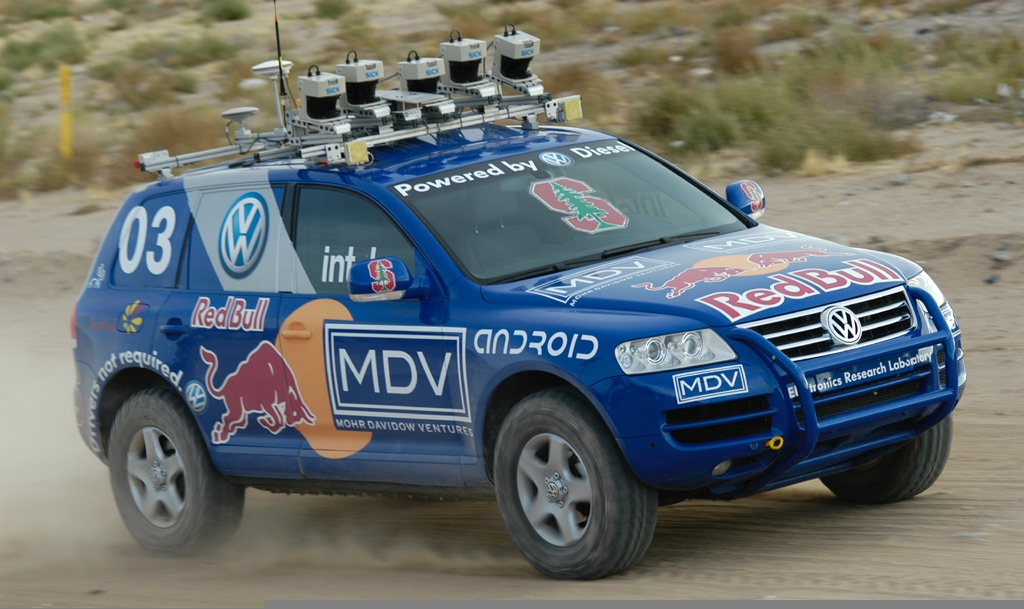
\includegraphics[width=0.5\textwidth]{img/stanley1}
\caption[Stanley]{Stanley, el vehículo autónomo de Stanford que ganó la competencia DARPA Grand Challenge en 2005. 
        Fuente: \href{http://stanford.edu/~cpiech/cs221/apps/driverlessCar.html}{stanford.edu} }
\label{fig:stanley1}
\end{figure}

El éxito de los proyectos que participaron en el grand challenge sentó un gran precedente en el desarrollo de lo que 
ahora se conoce como \textit{Self Driving Car} o vehículo autónomo. De hecho, muchos de los equipos 
participantes de este concurso se constituyen en la actualidad como existosas empresas de desarrollo o 
coadyuvan en iniciativas privadas de gigantes de la tecnología como Google, Uber o Nissan.

Sin embargo, debido al creciente interés tanto en investigación como económico en los sistemas de conducción 
autónoma, la Sociedad de Ingenieros en Automoción (SAE por sus siglas en inglés) ha elaborado un estándar donde se 
detallan distintos aspectos concernientes. La regulación define varios niveles de autonomía en 
vehículos terrestres, aéreos y acuáticos yendo desde un control completamente manual, 
normalmente observado en vehículos completamente mecánicos, pasando por asistencias al control 
hasta llegar a un vehículo completamente autónomo en todas sus tareas

% IMAGEN: niveles de autonomia
%%%% Figura 2 %%%%%%
\begin{figure}[!h] 
\centering
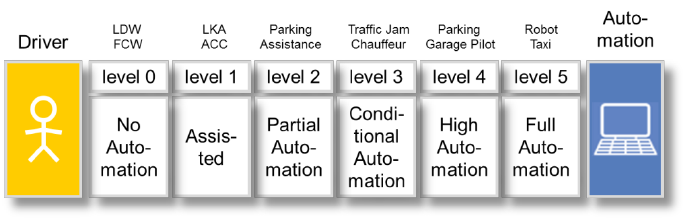
\includegraphics[width=0.70\textwidth]{img/levels}
\caption[Niveles de automatización SAE]{Niveles de automatización en la conducción según SAE. 
        Fuente: \href{https://www.researchgate.net/figure/Terms-related-to-automated-driving-according-to-SAE-and-VDA_fig1_273883061}{researchgate} }
\label{fig:levels}
\end{figure}

La creación de estándares y regulación ha tenido como consecuencia que, en la actualidad, existan varias iniciativas 
en el desarrollo de los \textit{self Driving Cars}, siendo una de las más 
importantes la empresa Waymo, dependiente de Google a través de su empresa Pública Alphabet. Waymo, ha aprovechado 
el uso de tecnologías emergentes de sensado como el LIDAR para mejorar el mapeo y la navegación a través de algoritmos 
de fusión de sensores. Aparte de Alphabet, existen diversas iniciativas privadas en el desarrollo de vehículos autónomos 
con fines comerciales como los Self Driving Cars de Uber, Toyota, BMW, Ford, entre otros.

% IMAGEN: vehiculo de waymo

%%%% Figura 1 %%%%%%
\begin{figure}[!h] 
\centering
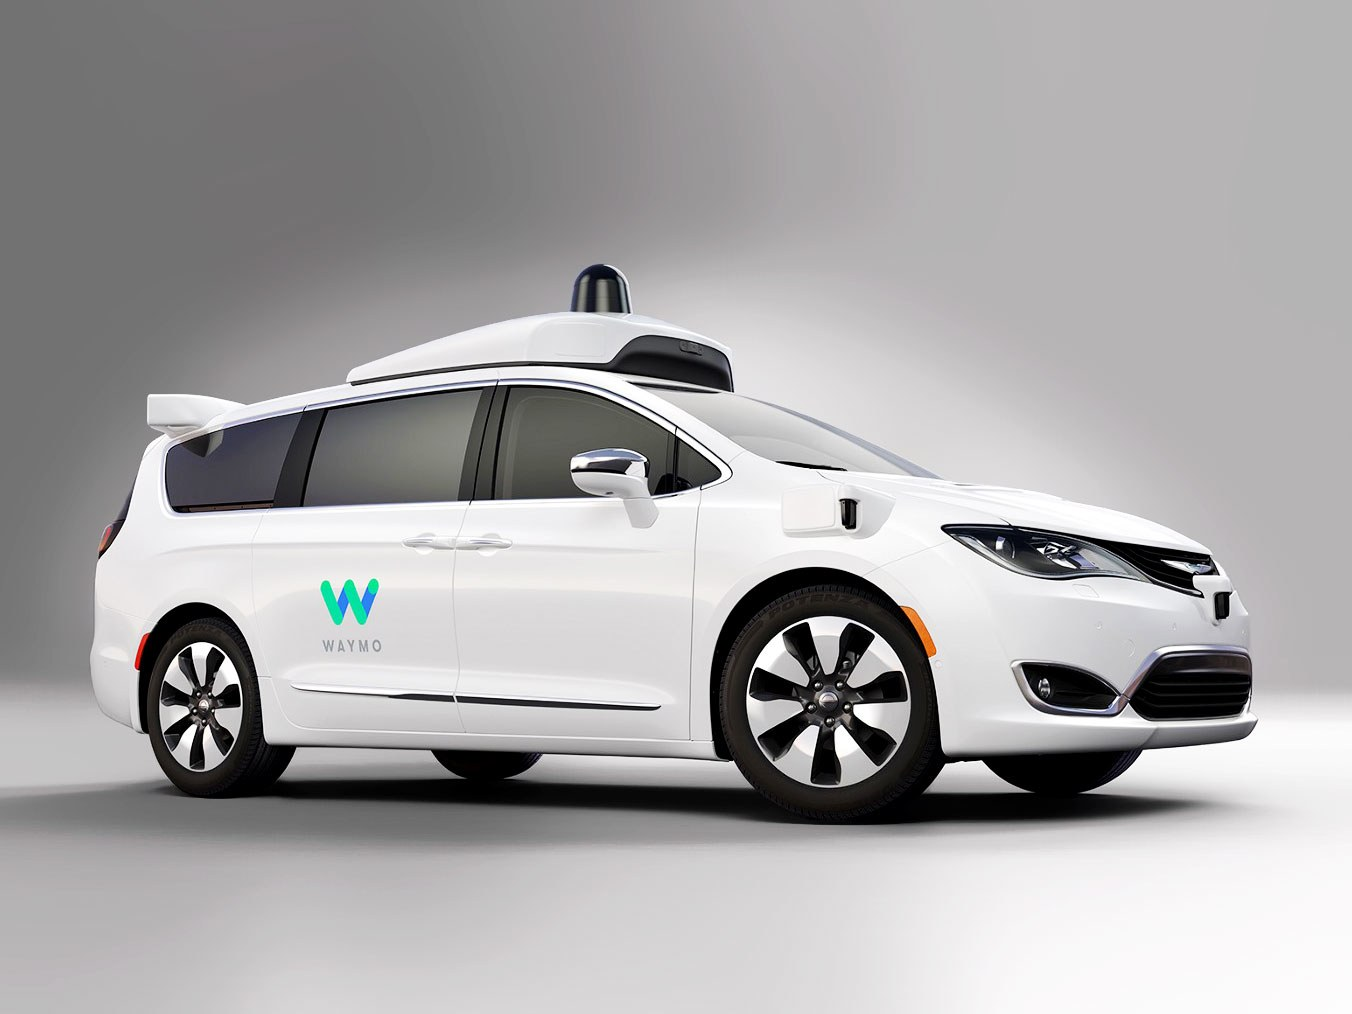
\includegraphics[width=0.5\textwidth]{img/waymo}
\caption[Vehículo de Waymo]{El vehículo autónomo de Waymo. 
        \href{https://waymo.com/}{waymo.com}}
\label{fig:waymo}
\end{figure}

Una de las tareas más importantes dentro de un \textit{self driving car} es la detección y mantención del carril del 
vehículo. Fabricantes de vehículos automotores han incluido con éxito sistemas de asistencia al conductor para la 
mantención del carril usando cámaras digitales y visión artificial para poder detectar la posición del automóvil con 
respecto al carril. Estos sistemas se consideran fundamentales en sistemas de conducción autónoma. Durante las últimas 
dos décadas, se han desarrollado distintos tipos de sistemas y enfoques para resolver el problema de la mantención de 
carril.

\subsubsection{Arquitectura general de un sistema de conducción autónoma}
En general, la arquitectura de un sistema de conducción autónoma se puede entender como la integración de varios módulos o 
subsistemas funcionales que operan en coordinación tal como se puede observar en la Figura(\ref{fig:esquema}). 

% IMAGEN: arquitectura

%%%% Figura 1 %%%%%%
\begin{figure}[!h] 
    \centering
    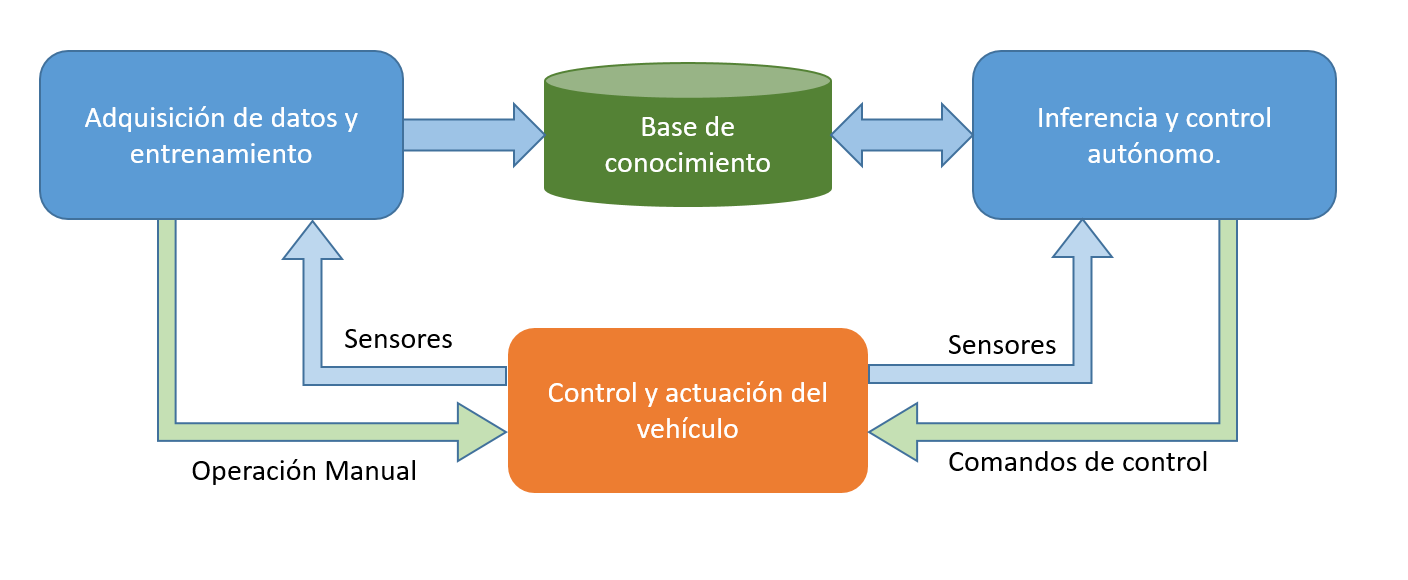
\includegraphics[width=0.75\textwidth]{img/esquema}
    \caption[Arquitectura de un sistema de conducción autónoma]{Arquitectura de un sistema de conducción autónoma. Fuente: Elaboración propia.}
    \label{fig:esquema}
\end{figure}


Normalmente, este tipo de sistemas cuenta con una etapa de adquisición de datos y entrenamiento que servirá para 
alimentar una base de conocimiento o reglas en las que se basará el módulo de inferencia y control autónomo. 
Asimismo, tanto el subsistema de adquisición de datos y entrenamiento como el subsistema de inferencia y 
control autónomo interactuan directamente con el subsistema de control y actuación del vehículo. 

Los mayores esfuerzos se han enfocado principalmente al desarrollo del subsistema de inferencia y 
control autónomo ya que es el que define el rendimiento de un sistema de conducción autónoma en sí. 
Este subsistema, a su vez, puede ser analizado como un conjunto de varios módulos que interactúan 
entre sí de manera secuencial, como se puede apreciar en la Figura(\ref{fig:inferencia}). 

\subsubsection{Sistemas de aprendizaje fin a fin}
Tradicionalmente, los sistemas de aprendizaje requieren de múltiples etapas de procesamiento que interactuan entre sí, como se 
muestra en la Figura(\ref{fig:inferencia}). Por su parte, los sistemas de aprendizaje fin a fin intentan condensar 
estas etapas de procesamiento y reemplazarlas usualmente con una sola red neuronal. Estos sistemas han demostrado ser 
altamente efectivos en contraste a los enfoques tradicionales, principalmente porque abstrae y resumen el diseño de las 
etapas intermedias de un sistema de aprendizaje tradicional con una sola etapa. La desventaja de los 
sistemas de aprendizaje fin a fin radica en la necesidad de grandes cantidades de datos de entrenamiento 
en comparación con los enfoques tradicionales, sin embargo, gracias a la gran disponibilidad de datos de entrenamiento y 
la accesibilidad de instrumentos y herramientas de adquisición de datos, esta desventaja no representa una dificultad de 
gran magnitud en el desarrollo de sistemas fin a fin. 

Los sistemas de aprendizaje fin a fin se han explorado de manera exitosa en los últimos años, esto debido a la creciente
disponibilidad de sistemas de cómputo de alta concurrencia, en especial las Unidades de Procesamiento Gŕafico de propósito
general o GPGPU por sus siglas en inglés. Esta disponibilidad ha logrado que se puedan entrenar redes neuronales completas 
en una estación de trabajo que no consume demasiada energía. Una de las empresas pioneras en GPGPU es Nvidia con su herramienta 
CUDA, que ha permitido el desarrollo de algoritmos de entrenamiento e inferencia para redes neuronales de manera sencilla. Es 
precisamente Nvidia que ha demostrado que los sistemas de aprendizaje fin a fin pueden tener éxito con el desarrollo de un 
prototipo y arquitectura de vehículo autónomo \cite{bojarski2016end}.


%*******************JUSTIFICACION*******************

\section{Justificación del Proyecto}

\subsection{Justificación académica}

Desde el punto de vista académico, el proyecto se justifica en el entendido del uso de técnicas y procedimientos 
de ingeniería para el análisis y diseño de un sistema de aprendizaje “fin a fin” usando redes neuronales y una plataforma 
para el entrenamiento y despliegue del mismo. Tales técnicas y procedimientos incluyen la definición de 
la arquitectura de la red neuronal, el entrenamiento y el análisis del rendimiento de la misma. Así como 
también el dimensionamiento de los componentes de cómputo embebido para el prototipo y la implementación de 
los sistemas de control electrónico de bajo nivel para el mismo. Tales técnicas y 
procedimientos se corresponden de manera integral con los conocimientos adquiridos a lo largo de la carrera 
de Ingeniería Electrónica en sus distintas asignaturas.

\subsection{Justificación tecnológica}

Dada la creciente relevancia de los sistemas autónomos en la actualidad, el proyecto se justifica 
desde el punto de vista tecnológico dado que se presenta la aplicación de nuevas
herramientas y plataformas de software para el desarrollo de sistemas de autónomos, visión por computador 
y redes neuronales convolucionales, que representan áreas vigentes en la investigación tecnológica hoy en día.

El sistema desarrollado se constituirá a su vez en una plataforma de desarrollo sobre el cual se podrá 
extender su funcionalidad y mejorar sus resultados usando herramientas de software de fácil acceso y aprendizaje 
presentando la posibilidad de continuar y extender la investigación en sistemas de conducción autónoma, robótica móvil, 
visión por computador y aprendizaje profundo.

\subsection{Justificación técnica}

Desde el punto de vista de las técnicas aplicadas, el proyecto se justifica dado que se pretende presentar una técnica 
alternativa al enfoque tradicional en el desarrollo de sistemas de aprendizaje, presentando el desarrollo de un sistema 
de aprendizaje fin a fin, que facilitará su análisis, diseño, entrenamiento y puesta en marcha en futuros proyectos 
de investigación y aplicaciones en distintas áreas de la ingeniería. 

La propuesta de la nueva técnica de aprendizaje fin a fin representa un avance en relación al desarrollo de sistemas 
tradicionales por su impacto en el requerimiento de recursos y de conocimiento específico requerido.


%******************ANALISIS DE LA PROBLEMATICA*********************
%------ TODO: completar esta parte ------------- %

\section{Análisis de la problemática y 
planteamiento del problema}
\subsection{Análisis de la problemática}
% PROBLEMATICA: Conjunto de aspectos que causan problemas en un PG.
% ANALISIS DE LA PROBLEMATICA: Determinacion de las causas sus efectos y sus relaciones, vinculados con los aspectos problematicos de la idea del proyecto.  
% ****Es el analisis de las cuestiones discutibles que requieren de una solucion en el PG.

Se han estudiado diferentes enfoques para lograr solucionar la tarea de 
conducción autónoma para vehículos domésticos usando sistemas de aprendizaje. Normalmente, la salida del 
sistema se expresa como una serie de comandos de control de aceleración y dirección 
del volante del vehículo. Estos comandos se pueden obtener de diversas maneras dependiendo 
el nivel de robustez y abstracción que el sistema requiere. Muchos sistemas 
se basan en la fusión de distintos tipos de sensores y fuentes de información como ser 
mapas satelitales, GPS, sensores láser y cámaras. La combinación de esta información 
es procesada y fusionada mediante distintos algoritmos de filtrado tales como el filtro de kalman. 
La característica de este tipo de sistema es que se puede expresar como una serie de etapas 
de procesamiento mediante el cual la información fluye y se transforma, cada una de las etapas es 
diseñada e implementada en base a conocimiento específico y con requerimientos y limitaciones específicas 
de la tarea que realiza tal como se puede apreciar en la Figura(\ref{fig:inferencia}).

Si bien el enfoque anteriormente mencionado ha logrado conseguir importantes avances y resultados 
muy prometedores, involucra un gran esfuerzo a la hora de diseñar cada una de las etapas independientemente 
para luego hacer que funcionen todas juntas y cumplan la tarea asignada. Este proceso usualmente requiere 
de un equipo de expertos que sea capaz de realizar las tareas de diseño de las etapas o módulos del sistema 
y el de la integración de los módulos en un solo sistema funcional. Este enfoque, pese a que ha demostrado ser 
una forma efectiva de trabajo para diversos problemas, tiene la desventaja de requerir muchos 
recursos y tiempo para poder lograr un sistema funcional. 

%
\subsection{Planteamiento del problema} \label{sec:problema}
% PLANTEAMIENTO DEL PROBLEMA: Tiene que ver con enfocar la solucion de los aspectos problematicos tratados, 
% desde su situacion inicial hasta su situacion final deseada.

% definir el concepto de informacion con referencia a datos
% 
De acuerdo a lo establecido anteriormente, se puede considerar a la etapa de inferencia y control autónomo de 
un sistema de conducción autónoma como un sistema de procesamiento de información que consta de varias etapas 
secuenciales que transforman la información de acuerdo a parámetros previamente establecidos. Se debe tener en 
cuenta varios aspectos concernientes tanto al diseño como a la implementación de dichos tipos de sistemas. 

%%%% Figura 1 %%%%%%
\begin{figure}[!h] 
    \centering
    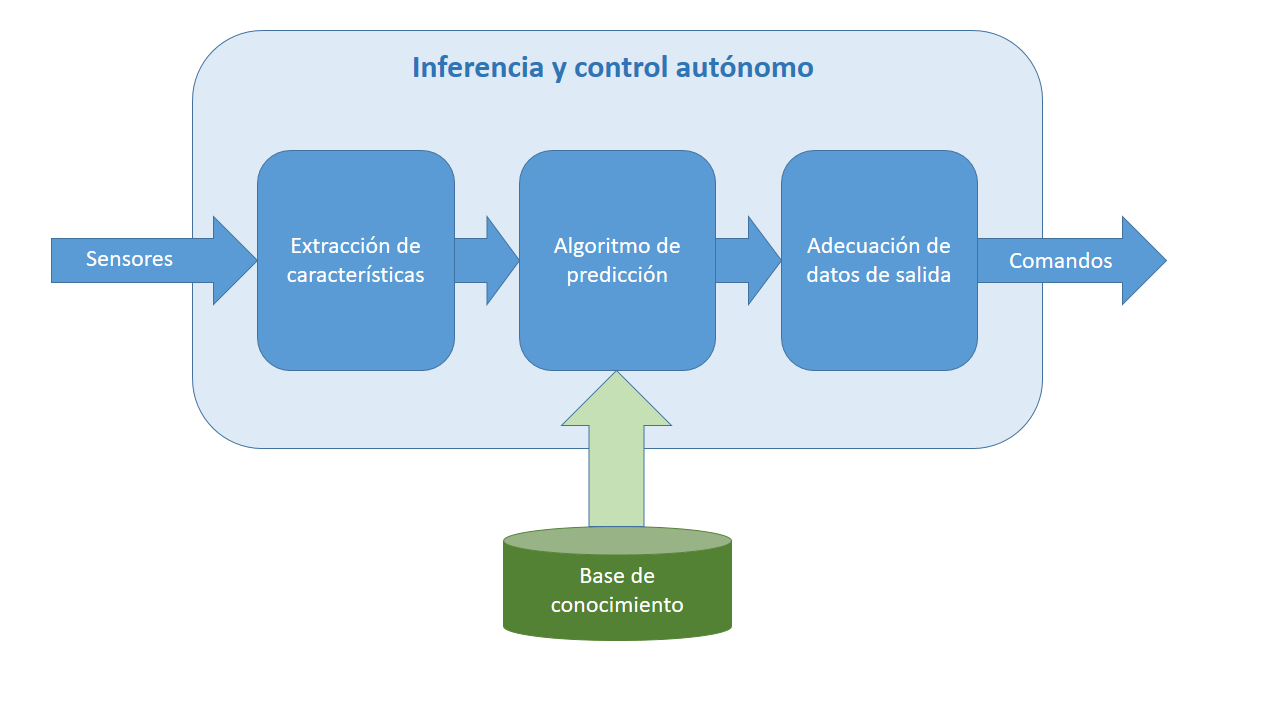
\includegraphics[width=0.75\textwidth]{img/inferencia}
    \caption[Inferencia y control autónomo tradicional]{Componentes del subsistema de inferencia y control autónomo tradicional. Fuente: Elaboración propia.}
    \label{fig:inferencia}
\end{figure}


En el área de visión por computadora para tareas de conducción autónoma, normalmente se sigue el siguiente 
flujo en el desarrollo un sistema o prototipo:

\begin{enumerate}
    \item \textbf{Extracción de características.} Esta etapa incluye el preprocesamiento y transformación de la imagen 
    en un conjunto de características de distinta índole. Estas características se suelen llamar también descriptores 
    y sirven para describir los aspectos más relevantes de la imagen para la tarea final, por ejemplo, la detección de bordes. 
    La extracción de características también se usa para reducir la dimensionalidad inicial de la imagen a una más tratable y 
    amigable con la capacidad de procesamiento computacional disponible. Las características o descriptores a usarse 
    se definen manualmente por medio de conocimiento experto y se afinan de la misma manera.

    \item \textbf{Algoritmo de predicción.} Esta etapa incluye típicamente un algoritmo de aprendizaje previamente 
    entrenado con un conjunto de datos adecuado, permite realizar distintas tareas de alto nivel sobre los descriptores 
    obtenidos de la imagen. Estas descripciones de alto nivel incluyen normalmente tareas de detección, 
    clasificación o regresión. Los algoritmos de aprendizaje incluyen típicamente algoritmos básicos, tales como árboles de decisión,
    regresión lineal o máquinas de soporte vectorial ya que deben realizar la tarea de predicción en un 
    conjunto de dimensionalidad relativamente baja (los descriptores).

    \item \textbf{Adecuación de los datos de salida.} La información extraída de la anterior etapa debe 
    procesarse para poder ser traducida a comandos de control que actuen directamente con las etapas 
    de bajo nivel del vehículo, es decir la etapa de actuación y potencia. En esta etapa se suele incluir algún algoritmo 
    de control realimentado para el control de motores así como también algoritmos de fusión de distintas fuentes de información
    para obtener finalmente una señal de comando para los actuadores.
\end{enumerate}

Como se ha podido observar, el flujo de trabajo en un sistema de conducción autónomo se compone de varias etapas 
secuenciales que se deben realizar con conocimiento y experiencia específica en cada una de las mismas. 

Por su parte, otra de las dificultades con este acercamiento, al reto de la conducción autónoma es el de la reducida
flexibilidad del sistema. En otras palabras, si se quisiera modificar el sistema para agregar requerimientos o 
expandir la funcionalidad del mismo, se debe realizar una modificación a la etapa específica y evaluar el impacto de 
las modificaciones en todo el sistema en su conjunto. Esto dificulta de manera sustancial la reutilización de diversos
componentes en sistemas similares.

Finalmente, la exagerada complejidad y conocimientos requeridos para poder implementar un sistema experimental 
de esta naturaleza hace prácticamente imposible su desarrollo por equipos de investigación pequeños o investigadores 
individuales. Dada la importancia y la potencialidad de los sistemas de conducción autónoma es escencial reducir 
esta dificultad de implementación y experimentación.

En conclusión, el desarrollo de un sistema de conducción autónoma presenta tres principales dificultades a la hora de 
ser abordado: 
\begin{enumerate}
    \item Conocimiento experto de cada una de las etapas involucradas en el sistema.
    \item Poca flexibilidad en el diseño y la implementación del sistema una vez establecido y probado.
    \item El tiempo y recursos necesarios para poder diseñar e implementar un sistema de tal naturaleza lo hace privativo para equipos de investigación pequeños o con poco presupuesto.
\end{enumerate}
%------------------
\section{Objetivos}
\subsection{Objetivo General}

Diseñar un sistema de aprendizaje “fin a fin” capaz de generar de comandos de 
control de vehículos domésticos basado en visión artificial y redes neuronales 
convolucionales para facilitar el diseño e implementación de sistemas de conducción autónoma.

\subsection{Objetivos Específicos}
Para alcanzar el objetivo general será necesario:


\begin{itemize}

    \item Estudiar los aspectos concernientes al desarrollo de sistemas de conducción autónoma y sistemas de aprendizaje.
    \item Analizar los requerimientos de un sistema de conducción autónoma capaz identificar y mantener su carril mientras se conduce.
    \item Diseñar la arquitectura de un sistema de conducción autónoma en base a los requerimientos previamente establecidos.
    \item Diseñar el subsistema de control y actuación para la conducción autónoma de un vehículo con características similares a las de un vehículo doméstico real.
    \item Diseñar el subsistema de adquisición de datos y entrenamiento para tareas de conducción autónoma.
    \item Diseñar el subsistema de inferencia y control autónomo basado en el uso de redes neuronales convolucionales.
    \item Analizar los resultados del entrenamiento e implementación del subsistema de inferencia y control autónomo.
    \item Realizar pruebas de rendimiento y análisis comparativos en el sistema implementado.

\end{itemize}


\section{Alcance}

El presente proyecto de grado cubre los siguientes aspectos dentro de su alcance:

\begin{itemize}
    \item El enfoque del estudio de sistemas de conducción autónomos de vehículos terrestres con el modelo de Ackermann.
    \item Investigación de arquitecturas y plataformas de software para el
    diseño y despliegue de robots móviles y tareas de conducción autónoma.
    \item El desarrollo del sistema se contempla en el marco de un proyecto académico 
    y, por tanto, será implementado usando herramientas de software comúnmente utilizadas en 
    investigación de sistemas autónomos.
\end{itemize}

El alcance detallado previamente estará acotado a su vez por una serie de supuestos.

\section{Límites}
El sistema, por su parte, contará con ciertas restricciones detalladas a 
continuación:
\begin{itemize}
    \item La tarea de conducción autónoma estará enfocada exclusivamente al 
    seguimiento y mantención del carril basado en imágenes provenientes de una cámara 
    sin considerar el reconocimiento e interpretación de otro tipo de información como 
    señales de tránsito, cruces e intersecciones o la presencia de peatones, ciclistas, 
    animales y otros objetos en la ruta.
    \item El prototipo a escala servirá solamente para un análisis superficial 
    de la dinámica de un vehículo automotor doméstico tomando como punto 
    de inicio modelos matemáticos simplificados y limitaciones de rangos de trabajo dentro 
    de dichos modelos.
    \item El diseño de la arquitectura de la red neuronal estará orientado a 
    tareas de aprendizaje supervisado y aproximación de funciones y limitado por la capacidad de 
    procesamiento disponible en el momento de la realización del presente proyecto.
\end{itemize}


\chapter{Marco Teórico} \label{ch:m_teorico}

% estructura
\section{Sistemas de Conducción Autónoma}
Un sistema de conducción autónoma es una combinación de varios componentes o subsistemas donde las tareas 
de percepción, toma de decisiones y operación de un vehículo son desarrolladas por un sistema electrónico en lugar
de un conductor humano. Usualmente, un sistema de conducción autónoma incluye varios subsistemas de automatización 
que operan de manera conjunta y coordinada para poder tomar el control total o parcial del vehículo. 

En algunas ocasiones, la automía del control se implementa de manera condicional, es decir, que el sistema toma 
el control del vehículo para ciertas situaciones pero no todo el tiempo como por ejemplo sistemas de estabilización 
de frenos o prevención de impactos. Este tipo de sistemas se ha ido desarrollando e implementando en vehículos comerciales 
de manera paulatina pero todavía no existe un vehículo completamente autónomo circulando por las calles o carreteras. Notese
que los términos autonomía y automatización se usan de manera intercambiable en este contexto.

Se han desarrollado tres enfoques concernientes al desarrollo de vehículos inteligentes de acuerdo al nivel de autonomía 
que presentan estos sistemas:

\begin{enumerate}
    \item \textbf{Enfoques centrados en el conductor.} Se diseñan en base a la idea de tener a un humano en el lazo de control 
    supervisando las funciones del vehículo
    \item \textbf{Enfoques centrados en una red.} Se diseñan con la idea de que los vehículos inteligentes puedan compartir información entre sí en una infraestructura de red.
    \item \textbf{Enfoques centrados en el vehículo.} Tienen el objetivo de desarrollar vehículos inteligentes completamente autónomos, sin la necesidad de la intervenión de un humano en el lazo de control.
\end{enumerate}

El interés en el desarrollo de vehículos completamente autónomos ha despertado el interés tanto de investigadores en todo 
el mundo así como también de instituciones privadas y gubernamentales que han invertido esfuerzos en fomentar éste desarrollo.
Una de las primeras instituciones en materializar una iniciativa en el desarrollo de vehículos autónomos fue la Agencia de Proyectos 
de Investigación Avanzados (DARPA, por sus siglas en inglés) con el lanzamiento del concurso \textit{Grand Challenge} en el 
año 2003 que era una carrera de vehículos autónomos que debían viajar por más de 200 Km en terrenos escabrosos. Este concurso sin 
sin precedentes atrajo la atención de un número de instituciones de investigación de alto nivel, lo que permitió que el desarrollo 
de este tipo de vehículos diera un gran paso adelante. 

En 2005, una nueva versión del DARPA \textit{Grand Challenge} requirió que los vehículos condujeran por una carretera en un 
desierto. En esta oportunidad, cinco vehículos completaron el trayecto de 211 Km en el desierto, con el vehículo de la Universidad 
de Stanford \textit{Stanley} como ganador, habiendo recorrido todo el trayecto en 6 horas con 54 minutos. En la Figura(\ref{fig:darpa}),
se pueden apreciar fotografías de los vehículos con mejor desempeño en la competencia.

El siguiente hito en el desarrollo de vehículos autónomos, fue el desarrollo del concurso organizado por DARPA 
\textit{Urban Challenge} en el año 2007, en el cual, los vehículos debían cumplir con ciertas tareas de 
navegación pero esta vez en un entorno urbano simulado, con avenidas, intersecciones, señalización y 
otros vehículos circulando simultáneamente. El recorrido comprendía aproximadamente 90 Km y representaba un reto por las 
complejas tareas de decisiones y comportamientos en un entorno de tráfico similar al que se puede encontrar cualquier conductor 
humano conduciendo en una ciudad. En esta ocasión, el ganador de la competencia fue el equipo Tartan Racing, un esfuerzo conjunto entre 
la Carnegie Mellon University y General Motors Corporation con el vehículo Boss, una versión modificada de un Chevrolet Tahoe.


\begin{figure}[!h] 
    \centering
    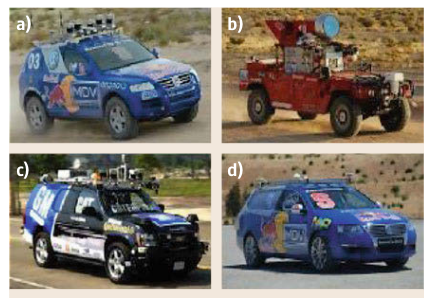
\includegraphics[width=0.75\textwidth]{img/darpa}
    \caption{Vehículos del \textit{Grand Challenge} de 2005: (a) Stanley (1er lugar), (b) Sandstorm (2do lugar). Vehículos del \textit{Urban Challenge} de 2007: (c) Boss (1er lugar) (d) Junior (2do lugar). Fuente: \cite{wikipedia_2018} }
    \label{fig:darpa}
\end{figure}



    \subsection{Niveles de Autonomía SAE}
    Debido al creciente interés e inversión en el desarrolo de sistemas de conducción autónoma se ha establecido 
    una manera de categorizar los niveles de automatización de la conducción por parte de  la Sociedad de Ingenieros en Automoción
    (SAE, por sus siglas en inglés) en la que se definen seis niveles de automatización en vehículos terrestres, acuáticos y aéreos.

        \subsubsection{Nivel 0: Sin automatización}
        El conductor está en completo control de todas las funciones del vehículo en todo momento, no existe intervención 
        de ningún sistema automatizado en el control. Sistemas de alerta de colisión o pérdida de carril entran en esta categoría.
        
        \subsubsection{Nivel 1: Conducción asistida}
        El conductor tiene el control del vehículo, pero el sistema puede modificar la aceleración o dirección del mismo. Los 
        sistemas de control de velocidad de crucero caen en esta categoría.
        
        \subsubsection{Nivel 2: Automatización parcial}
        El conductor debe poder ser capaz de tomar el control del vehículo si ciertas se necesitan ciertas correcciones, pero  
        ya no está en control de la aceleración y dirección del vehículo directamente. Es importante resaltar que desde los
        niveles 0 al 2 el conductor no puede estar distraido en ningún momento de la conducción. Los sistemas de parqueo 
        automático representan un buen ejemplo de sistemas de Nivel 2.
        
        \subsubsection{Nivel 3: Automatización condicional}
        El sistema automatizado tiene el control del vehículo, tanto de la aceleración, dirección así como también del monitoreo 
        del entorno bajo condiciones específicas. El conductor debe estar preparado para intervenir cuando el sistema así lo 
        requiera, por tanto, se permiten distracciones ocasionales. Uno de los sistemas recientemente implementados que cae en esta 
        categoría es el sistema \textit{autopilot} de los vehículos de Tesla Motors. % agregar referencia
        
        \subsubsection{Nivel 4: Automatización elevada}
        El sistema está en completo control del vehículo y la presencia humana ya no es necesaria, sin embargo, la operación autónoma 
        del vehículo está limitada a condiciones específicas. Si las actuales condiciones del entorno sobrepasan las fronteras 
        de rendimiento definidas, el vehículo puede desplegar un protocolo o secuencia de emergencia. Actualmente el desarrollo 
        de vehículos autónomos o \textit{self driving cars} se enfoca en este nivel. 
        
        \subsubsection{Nivel 5: Automatización completa}
        El sistema está en completo control del vehículo y la presencia humana no es necesaria en absoluto. El sistema es capaz 
        de proveer las mismas características que en el Nivel 4, pero en esta ocasión puede operar al vehículo en todas las condiciones.
        En este nivel, el conductor pasa a ser un pasajero en el vehículo. Actualmente, no existen sistemas que operen en este nivel.

    La relación entre la responsabilidad del sistema y el conductor en los distintos niveles se puede apreciar en la 
    Tabla \ref{tbl:niveles}:
    
        \begin{table}[!h]
            \centering
            \resizebox{\textwidth}{!}{%
            \begin{tabular}{@{}|c|l|c|c|c|c|@{}}
            \toprule
            \textbf{Nivel SAE} & \textbf{Denominación}      & \textbf{\begin{tabular}[c]{@{}l@{}}Ejecución de aceleración \\ y dirección\end{tabular}} & \textbf{\begin{tabular}[c]{@{}l@{}}Monitoreo del \\ entorno\end{tabular}} & \textbf{\begin{tabular}[c]{@{}l@{}}Responsable en \\ condiciones difíciles\end{tabular}} & \textbf{\begin{tabular}[c]{@{}l@{}}Modos de \\ conducción\end{tabular}} \\ \midrule
            0                  & Sin Automatización         & Humano                                                                                   & \multirow{3}{*}{Humano}                                                   & \multirow{4}{*}{Humano}                                                                  & Ninguno                                                                 \\ \cmidrule(r){1-3} \cmidrule(l){6-6} 
            1                  & Conducción asistida        & Humano y sistema                                                                         &                                                                           &                                                                                          & \multirow{3}{*}{Algunos Modos}                                          \\ \cmidrule(r){1-3}
            2                  & Automatización parcial     & \multirow{4}{*}{Sistema}                                                                 &                                                                           &                                                                                          &                                                                         \\ \cmidrule(r){1-2} \cmidrule(lr){4-4}
            3                  & Automatización condicional &                                                                                          & \multirow{3}{*}{Sistema}                                                  &                                                                                          &                                                                         \\ \cmidrule(r){1-2} \cmidrule(l){5-6} 
            4                  & Automatización elevada     &                                                                                          &                                                                           & \multirow{2}{*}{Sistema}                                                                 & Varios Modos                                                            \\ \cmidrule(r){1-2} \cmidrule(l){6-6} 
            5                  & Automatización completa    &                                                                                          &                                                                           &                                                                                          & Todos los Modos                                                         \\ \bottomrule
            \end{tabular}%
            }
            \caption{Niveles de automatización según SAE. Fuente: SAE} % TODO: referencia
            \label{tbl:niveles}
            \end{table}

    
    \subsection{Tecnologías requeridas}
    Las tecnologías básicas para sensado y actuación para vehículos autónomos ya existen en el mercado. El reto clave es el 
    de integrar dichas tecnologías con nuevos desarrollos en un sistema estable. Para poder desarrollar sistemas de conducción 
    autónoma confiables y seguros se necesita lo siguiente:

    \begin{itemize}
        \item Una forma de medir o estimar el estado del vehículo.
        \item Una forma de medir o estimar el estado del entorno en el que el vehículo circula.
        \item Acceso a mapas e información satelital.
        \item Una infraestructura de comunicación distribuida con otros vehículos.
    \end{itemize}

        \subsubsection{Estado del vehículo}
        La localización del vehículo es fundamental para tareas de conducción autónoma y debe ser conocida si se desea que siga 
        una trayectoria definida. Para controlar un vehículo de forma que sea capaz de evadir obstáculos o mantener un carril, se 
        necesita conocimiento del estado cinemático y dinámico del mismo. Diversas fuentes de información y datos sobre el estado
        del vehículo pueden ser incorporados como encoders, o unidades inerciales en combinación con medidas de navegación absolutas 
        como GPS. Adicionalmente, la posición del vehículo puede ser conocida con referencia a marcadores locales. Aparte de la 
        localización del vehículo, sistemas de medición de parámetros internos y control de funciones como aceleración, dirección 
        estado del motor, y otros, pueden ser incorporados.

        El desarrollo de modelos adecuados para el control del vehículo también representa una tarea importante pues es en 
        base a estos modelos sobre los cuales se desarrollarán los algoritmos que lo controlen. 

        \subsubsection{Estado del entorno}
        Otro aspecto crítico en el desarrollo de un sistema autónomo es el sensado del estado del entorno y cómo el mismo 
        evoluciona en el tiempo. La tarea más difícil para un vehículo es poder generar un entendimiento de lo que pasa en 
        la carretera, esto incluye poder detectar marcadores clave, otros vehículos, peatones, la carretera o avenida por la que 
        esta circulando actualmente y otros obstáculos como árboles. 
        
        La información se obtiene de diversos tipos de sensores 
        montados en el mismo vehículo, de los cuales los más comunes son los sensores visuales o cámaras que pueden ser posicionadas 
        en distintas orientaciones para poder observar todo lo que ocurre alrededor del vehículo. Los datos de las cámaras 
        son procesados con el objetivo de extraer información valiosa como la ubicación del carril, detección de peatones y otros 
        obstáculos. Otro tipo de sensores utilizados comunmente son sensores de proximidad, que permiten obtener medidas de distancia 
        a los obstáculos más cercanos ofreciendo así información al vehículo sobre su posición relativa a los mismos. 
        
        Un tipo especial de sensores muy comunes en vehículos autónomos son los LIDAR, que generan una nube de puntos 
        con información acerca de la distancia a los obstáculos más cercanos en dos y tres dimensiones.
        % imagen de lidar 
        \begin{figure}[!h] 
            \centering
            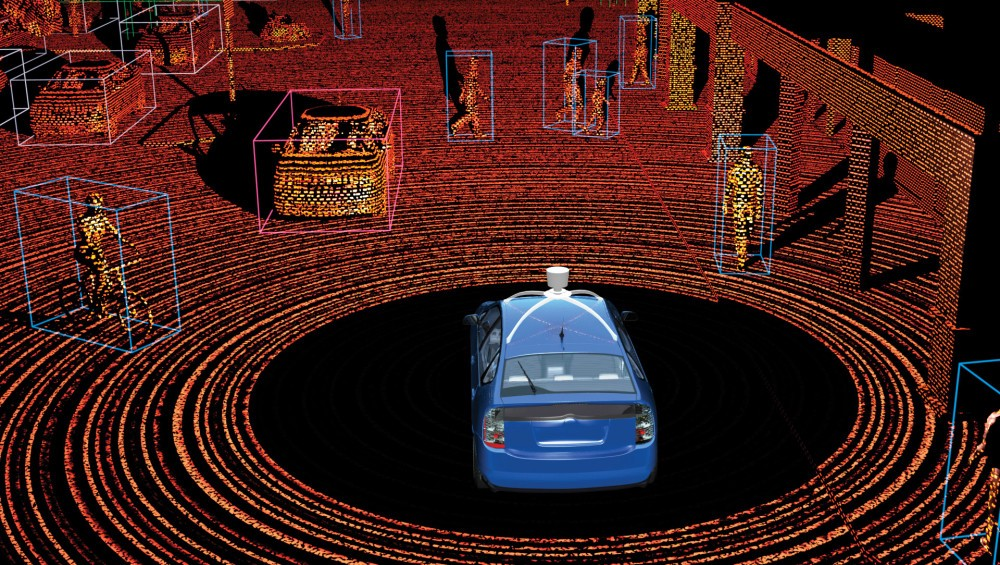
\includegraphics[width=0.75\textwidth]{img/lidar}
            \caption{Visualización de los datos provenientes de un LIDAR para tareas de conducción autónoma. Fuente: \cite{cameron_2017} }
            \label{fig:lidar}
        \end{figure}
        

    \subsection{Arquitectura de un sistema de conducción autónoma}
    En base a los distintos aspectos detallados anteriormente (Figura(\ref{fig:esquema})), en el marco de los objetivos del presente 
    proyecto, se puede describir a la tarea de conducción autónoma usando una arquitectura compuesta 
    por tres elementos o subsistemas fundamentales: el subsistema de control y actuación del vehículo, el 
    subsistema de adquisición de datos y entrenamiento y el subsistema de inferencia y control.

        \subsubsection{Subsistema de control y actuación.}
        Este subsistema representa la parte física y de bajo nivel del vehículo, el vehículo en sí, 
        sumado a los sistemas de control y sensado incorporados. Este subsistema cuenta con las interfaces necesarias 
        para controlar el vehículo mediante comandos de control de aceleración y dirección y con los medios 
        para extraer información del estado interno del vehículo, así como también del entorno con cámaras o sensores 
        de proximidad. Por sí solo, este subsistema no es capaz de realizar ninguna tarea de conducción autónoma.

        % TODO: grafico del subsistema
        \subsubsection{Subsistema de adquisición de datos y entrenamiento.}
        Este subsistema se compone de un conjunto de herramientas y utilidades para la 
        adquisición de conjuntos de datos de entrenamiento y validación, así como
        también un módulo de entrenamiento de la red neuronal convolucional para la tarea de
        la generación de comandos de control. En la parte de adquisición de datos, provee de las herramientas necesarias 
        para poder extraer información relevante de sesiones de conducción controlada por un operador humano de forma 
        que se tengan los datos necesarios para que el vehículo pueda aprender la forma de conducir en base a una referencia 
        de conducción humana.

        \subsubsection{Subsistema de inferencia y conducción autónoma.}
        El subsistema de inferencia y conducción autónoma tiene la tarea de obtener y ejecutar
        las predicciones del modelo predictivo entrenado en el Subsistema de Adquisición de Datos y Entrenamiento.
        Este subsistema tomará como entradas los datos de los 
        sensores a bordo del vehículo para generar comandos de control acordes con el entorno
        percibido. Este subsistema usualmente está implementado en forma de un programa de ``piloto automático''
        capaz de conducir el prototipo de manera autónoma de acuerdo a las limitaciones definidas en el diseño.

\section{Visión Artificial}
La visión es un sentido fundamental en el desarrollo de cualquier persona y, entender el entorno basados en la información que 
un humano puede ver es relativamente sencillo. Tareas como reconocer la forma y color de un objeto cercano o contar las personas 
presentes en una fotografía de grupo son tareas triviales para un ser humano. La visión artificial es un campo de 
las ciencias de la computación que intenta reproducir las capacidades de una persona para entender imágenes. Este campo
aglutina técnicas matemáticas para recuperar la forma y apariencia en tres dimensiones de objetos en una imagen. Se trata 
del desarrollo de distintas técnicas y algoritmos que intentan recuperar la información más importante de una imagen digital, 
en otras palabras, que una computadora pueda entender una imagen. En la actualidad, las técnicas de visión artificial son 
usadas en diversas aplicaciones de la vida real de las cuales podemos citar algunas:

\begin{itemize}
    \item \textbf{Reconocimiento optico de caracteres (OCR):} Lectura de dígitos manuscritos de códigos postales (Figura(\ref{fig:cvision}a)) y reconocimiento automático de placas de vehíchulos.
    \item \textbf{Inspección automática:} Inspección de partes para el control de calidad en líneas de producción industriales(Figura(\ref{fig:cvision}b)).
    \item \textbf{Ventas:} Reconocimiento de objetos para pagos en cajas automatizadas(Figura(\ref{fig:cvision}c)).
    \item \textbf{Reconstrucción de modelos en 3D (fotogrametría):} Reconstrucción automática de modelos en tres dimensiones a partir de fotografías aéreas.
    \item \textbf{Imagenología médica:}  Registro de imágenes pre y post operatorias para estudios y diagnósticos especializados(Figura(\ref{fig:cvision}d)).
    \item \textbf{Seguridad automotriz:} Detección de obstáculos inesperados como peatones o ciclistas en situaciones donde métodos convencionales de detección de obstáculos no pueden aplicarse (Figura(\ref{fig:cvision}e)).
    \item \textbf{Seguridad y vigilancia:} Monitoreo de actividad sospechosa y análisis de tráfico en carreteras (Figura(\ref{fig:cvision}f)).
\end{itemize}


\begin{figure}[!h] 
    \centering
    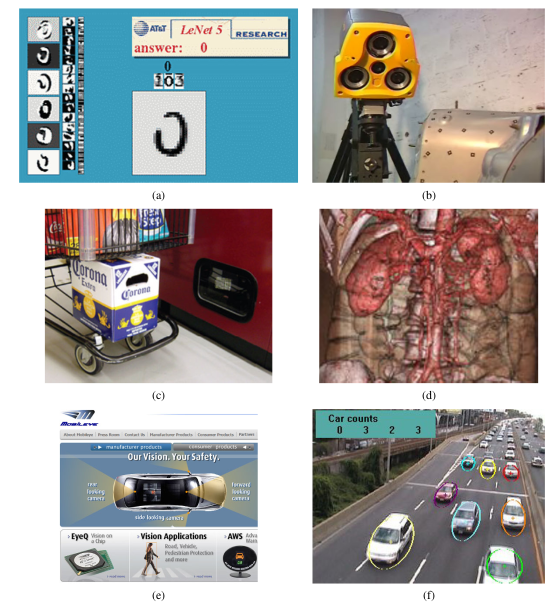
\includegraphics[width=0.75\textwidth]{img/cvision}
    \caption{Algunas aplicaciones de la visión artificial. Fuente: \cite{Szeliski2011} }
    \label{fig:cvision}
\end{figure}

    \subsection{Caracterización de una imagen digital}
    Luego de surgir de una o más fuentes de luz, reflejarse de una o más superficies y pasar a través del lente de una cámara, 
    la luz finalmente llega al sensor óptico. Los fotones incidentes en el sensor son convertidos en valores de intensidad de 
    color rojo, verde y azul (RGB) en un arreglo matricial que es lo que se conoce como una imagen digital. Todas las etapas 
    envueltas en la obtención de una imagen digital se pueden apreciar en la Figura(\ref{fig:digitalcam}) donde se diferencian 
    dos subproductos del proceso de conversión: la imagen \textit{raw} y la imagen compresa. Esta diferenciación nace de la 
    necesidad de representar imágenes digitales sin ocupar mucho espacio en la memoria y para poder comprimir una imagen 
    \textit{raw} se realizan varios procesos complementarios.

    \begin{figure}[!h] 
        \centering
        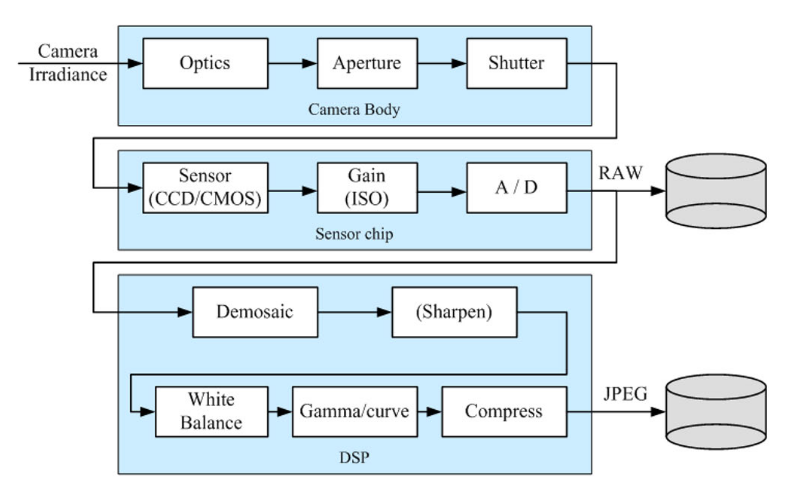
\includegraphics[width=0.75\textwidth]{img/digitalcam}
        \caption{Proceso de la obtención de una imagen con una cámara digital. Fuente: \cite{Szeliski2011} }
        \label{fig:digitalcam}
    \end{figure}

    El sensor óptico se compone de un arreglo bidimensional de pixeles sensibles a la luz y a ciertos rangos de longitud de onda de 
    la luz, lo que significa que pueden detectar ciertos colores o características de la luz que incide en ellos. Este arreglo 
    se transforma en una matriz con valores de intensidad para cada color en cada pixel, es así como se puede entender 
    a una imagen digital como un arreglo multidimensional de valores. 

    \begin{figure}[!h] 
        \centering
        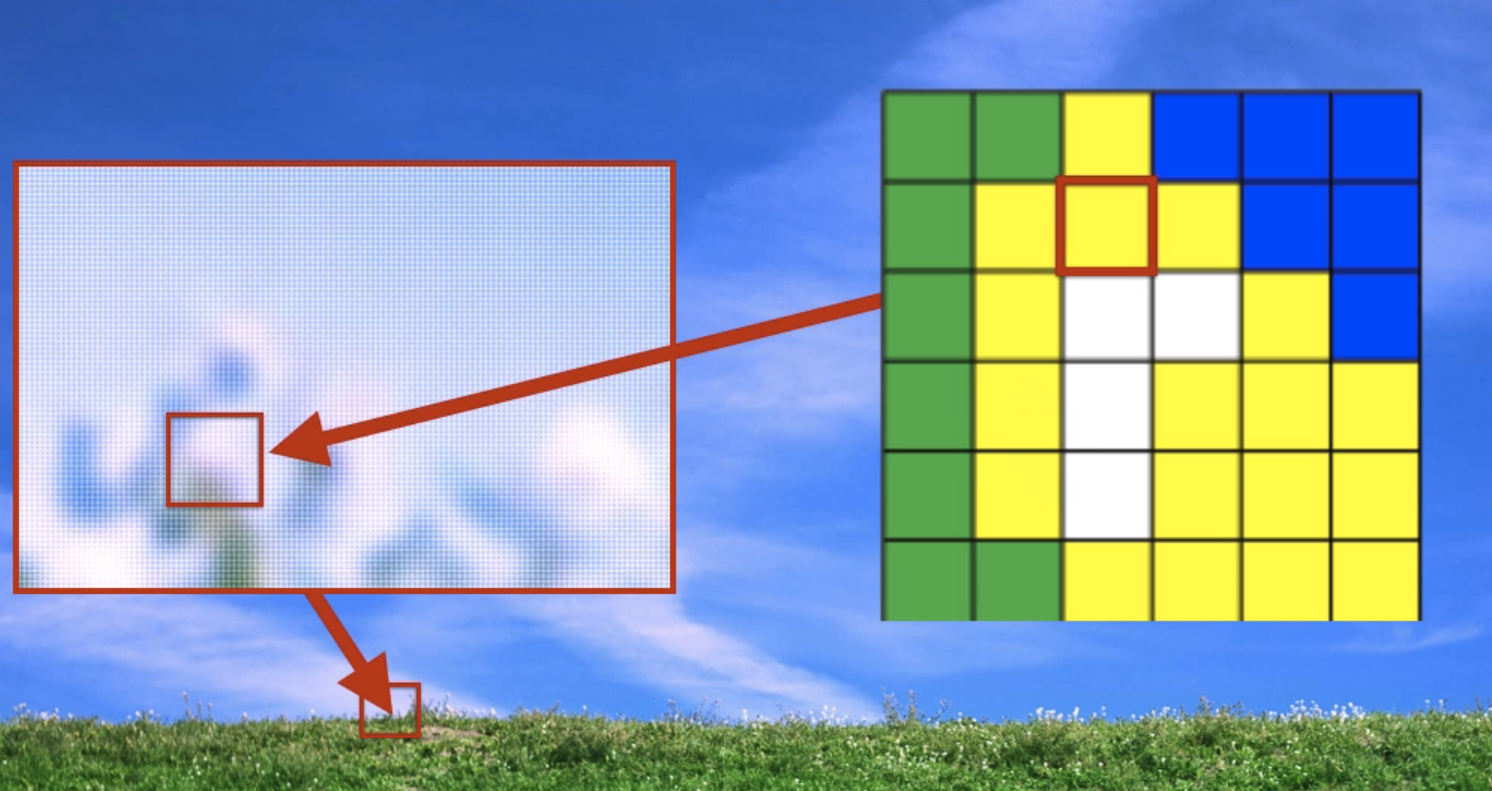
\includegraphics[width=0.75\textwidth]{img/digitalimg}
        \caption{Representación de una imagen digital como un arreglo de pixeles. Fuente: \cite{Szeliski2011} }
        \label{fig:digitalimg}
    \end{figure}

    La tarea de la visión artificial es especialmente complicada pues se intenta dar sentido o significado a un arreglo bidimensional 
    de pixeles. Existen distintos métodos y algoritmos que intentan convertir esta inmensa cantidad de datos (los pixeles) en 
    información útil (objetos).

\section{Redes Neuronales Artificiales}         %done

    \subsection{Aprendizaje Automático}
    El aprendizaje automático es un subcampo de la inteligencia artificial que intenta extraer 
    patrones mediante un proceso de \textit{aprendizaje} a partir de datos \cite{Mitchell1990}. Este proceso 
    de aprendizaje se define de acuerdo a una \textbf{tarea específica} $T$ que intenta aprenderse en base 
    a \textbf{experiencia pasada} $E$ tomando como referencia una \textbf{medida de rendimiento} $P$ . 
    Dentro de esta definición, se puede listar varios ejemplos de tareas de aprendizaje que usualmente se resuelven  
    usando los conceptos del aprendizaje automático o también llamado \textit{machine learning}:
    \\
    \\
    \begin{itemize}
        \item \textbf{Un algoritmo de aprendizaje que pueda jugar ajedrez:}
        \begin{itemize}
            \item \textbf{Tarea $T$:} Jugar Ajedrez.
            \item \textbf{Medida de Rendimiento $P$:} Porcentaje de partidas ganadas contra el oponente.
            \item \textbf{Experiencia $E$:} Información de varias partidas de práctica.
        \end{itemize}
        
        \item \textbf{Un algoritmo de aprendizaje que pueda reconocer dígitos manuscritos:}
        \begin{itemize}
            \item \textbf{Tarea $T$:} Reconocer y clasificar dígitos manuscritos dentro de una imagen.
            \item \textbf{Medida de Rendimiento $P$:} Porcentaje de dígitos correctamente clasificados.
            \item \textbf{Experiencia $E$:} Base de datos de imágenes de dígitos con sus etiquetas correspondientes.
        \end{itemize}

        \item \textbf{Un algoritmo de aprendizaje que pueda reconocer la voz:}
        \begin{itemize}
            \item \textbf{Tarea $T$:} Extraer una secuencia de palabras de una grabación de voz.
            \item \textbf{Medida de Rendimiento $P$:} Porcentaje de palabras correctamente predichas.
            \item \textbf{Experiencia $E$:} Grabaciones de voz con una transcripción correspondiente.
        \end{itemize}
    
    \end{itemize}
    

    Esta definición de aprendizaje es lo suficientemente amplia como para englobar todas las tareas 
    que el campo del aprendizaje automático intenta resolver en la actualidad. Sin embargo, debido a 
    su naturaleza, se pueden clasificar las tareas de aprendizaje en tres grandes categorías que tienen
    características particulares: aprendizaje supervisado, aprendizaje no supervisado y aprendizaje por refuerzo.

    La diferencia entre estos tres tipos de problemas surge de la distinta naturaleza de la experiencia $E$ disponible
    para el entrenamiento. A continuación, se procede a detallar cada uno de ellos.

        \subsubsection{Aprendizaje supervisado} \label{sss:supervisado}
        En el caso de las tareas de aprendizaje supervisado, la experiencia constituye un conjunto de datos o \textit{dataset}
        que contiene ejemplos con \textit{características} y cada ejemplo está asociado con una \textit{etiqueta}. Por ejemplo, 
        un conjunto de datos de flores donde cada registro contiene datos de la flor (características) y la especie a la que pertenece (etiqueta). 
        Dentro de los algoritmos que atacan problemas de aprendizaje supervisado se pueden encontrar 2 grandes categorías.
            \paragraph{Clasificación}
            Las tareas de clasificación tienen como característica el hecho de que la etiqueta de cada ejemplo en el 
            conjunto de datos pertenece a una categoría o, en otras palabras, tiene una naturaleza discreta y finita. Por ejemplo, 
            en el caso de la clasificación de las flores mencionado anteriormente, la etiqueta solamente puede pertenecer a un
            conjunto finito de especies de flores y cada ejemplo pertenece a una de estas especies.
            \paragraph{Regresión}
            En las tareas de regresión, las etiquetas pertenecen a un conjunto de números reales o de naturaleza 
            contínua. En este caso, las etiquetas no se asocian con categorías sino más bien con otro tipo de variables. Un 
            ejemplo muy conocido es el de la tarea de la predicción del precio de una casa en base a sus características, el precio 
            de una casa no puede categorizarse porque representa un número que puede tener infinitos valores dentro de un rango definido.
        

            \begin{figure}[!h] 
                \centering
                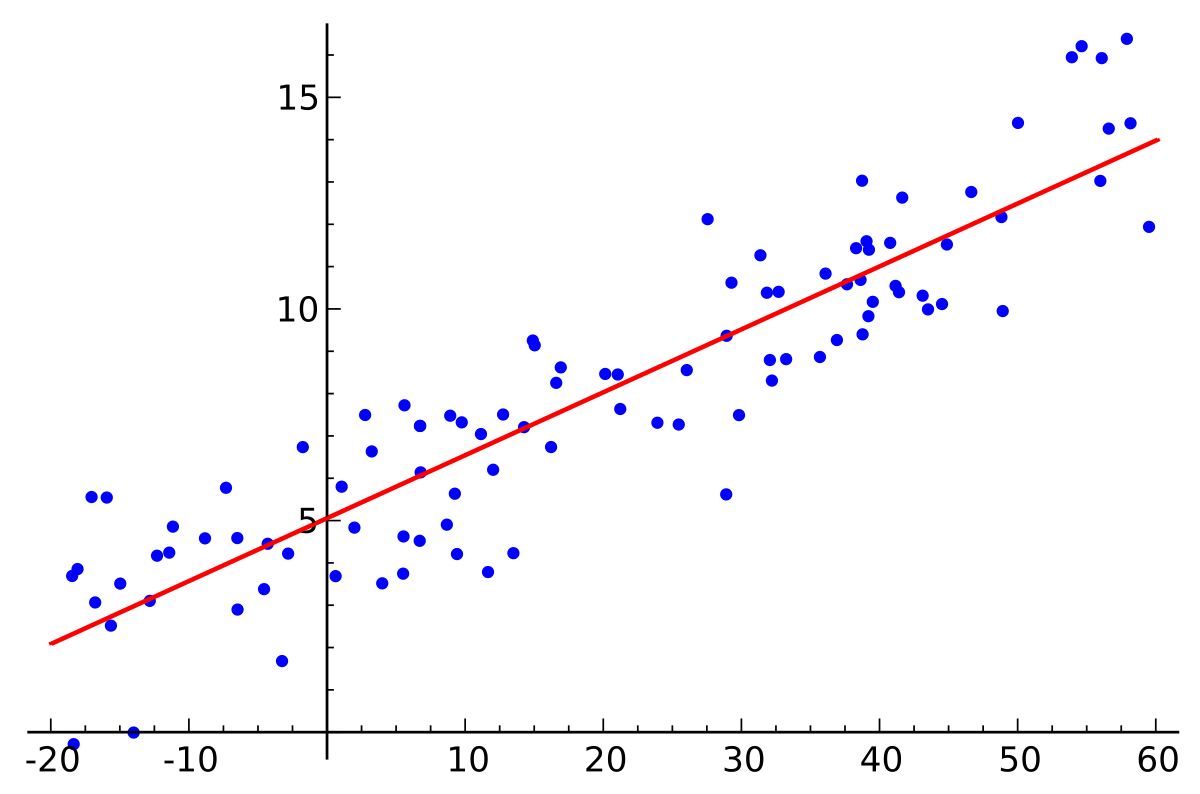
\includegraphics[width=0.75\textwidth]{img/regression}
                \caption{Regresión lineal, una tarea de aprendizaje supervisado. Fuente: \cite{wikipedia_2018} }
                \label{fig:regresion}
            \end{figure}

        En las tareas del aprendizaje supervisado, se puede considerar cada ejemplo como una descripción de 
        una situación (características) en conjunto con una especificación (etiqueta), cada uno de los ejemplos 
        dentro el conjunto de datos son eventos independientes y se pueden analizar por separado. En este sentido
        la tarea del algoritmo es generalizar la respuesta para casos no presentes en el conjunto inicial de datos.

        \subsubsection{Aprendizaje no supervisado}
        En las tareas del aprendizaje no supervisado la experiencia contenida en el conjunto de datos tiene la característica de 
        no poseer ninguna etiqueta, por tanto, usualmente se intenta buscar una estructura escondida dentro el conjunto de datos 
        o, dicho de otra manera, se buscan patrones que puedan presentarse en dichos datos. Estos patrones pueden aprovecharse 
        para extraer información relevante de la naturaleza de datos de muy alta dimensionalidad, información que normalmente no 
        es trivial de encontrar o visualizar por una persona. Entre algunas de las tareas más comunes dentro del aprendizaje no 
        supervisado, se pueden listar:

            \paragraph{Clustering}
            Refiere a la tarea de separar y agrupar los datos en un número finito de conjuntos o \textit{clusters}. Los 
            \textit{clusters} normalmente denotan una estructura oculta dentro de los datos y proporcionan información acerca 
            de la similaridad entre ejemplos del conjunto de datos.

            \begin{figure}[!h] 
                \centering
                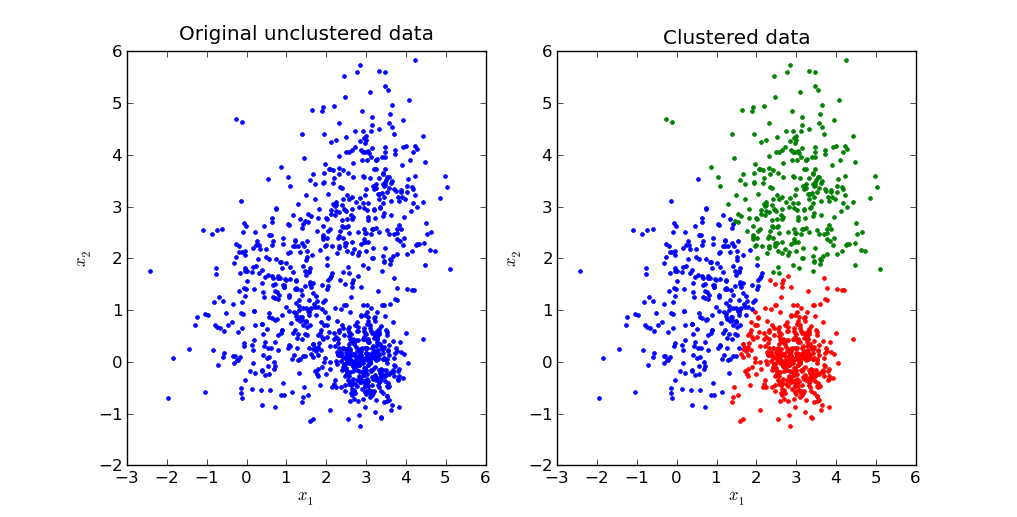
\includegraphics[width=0.75\textwidth]{img/clustering}
                \caption{Clustering, una tarea de aprendizaje no supervisado. Fuente: \cite{viswarupan_2017} }
                \label{fig:clustering}
            \end{figure}

            \paragraph{Reducción de dimensionalidad}
            Uno de los problemas con las bases de datos y conjuntos de datos disponibles es que poseen una dimensionalidad 
            bastante alta haciendo prácticamente imposible para un humano poder visualizar o encontrar patrones e información 
            útil en los mismos. Este problema se suele tratar con algoritmos de reducción de dimensionalidad, en la que 
            se encuentra una representación estimada de los datos pero con menos dimensiones. Uno de los algoritmos más 
            conocidos y usados en esta categoría es el análisis de componente principal o PCA, por sus siglas en inglés, en el 
            que se encuentra una representación de los datos en una menor dimensión usando proyecciones ortogonales.

            \paragraph{Estimación de probabilidad}
            Muchos conjuntos de datos son obtenidos de distintas fuentes y a lo largo de varios intervalos de tiempo, en este 
            entendido, es muy útil conocer o aproximar la distribución de probabilidad de los datos para luego poder realizar 
            predicciones o tratarlos con algún modelo en específico.

        \subsubsection{Aprendizaje por refuerzo}
        En las tareas de aprendizaje por refuerzo se toma en cuenta la interacción de un agente con su entorno y la forma 
        en la que las acciones que toma dicho agente afectan a su entorno y se materializan en una recompensa o castigo \cite{sutton2018reinforcement}. Formalmente
        se pueden definir ciertos elementos que componen una tarea de aprendizaje por refuerzo:
        \begin{itemize}
            \item \textbf{Agente.} Es la entidad que interactúa con el entorno. El agente se comunica con el entorno mediante acciones.
            \item \textbf{Política.} Representan la forma de actuar del agente en base al conocimiento que ha adquirido.
            \item \textbf{Recompensa.} Es la función que define la efectividad del agente de cumplir el objetivo deseado, normalmente, el aprendizaje se enfoca en maximizar la recompensa que el agente puede obtener. 
        \end{itemize}
        
        \begin{figure}[!h] 
            \centering
            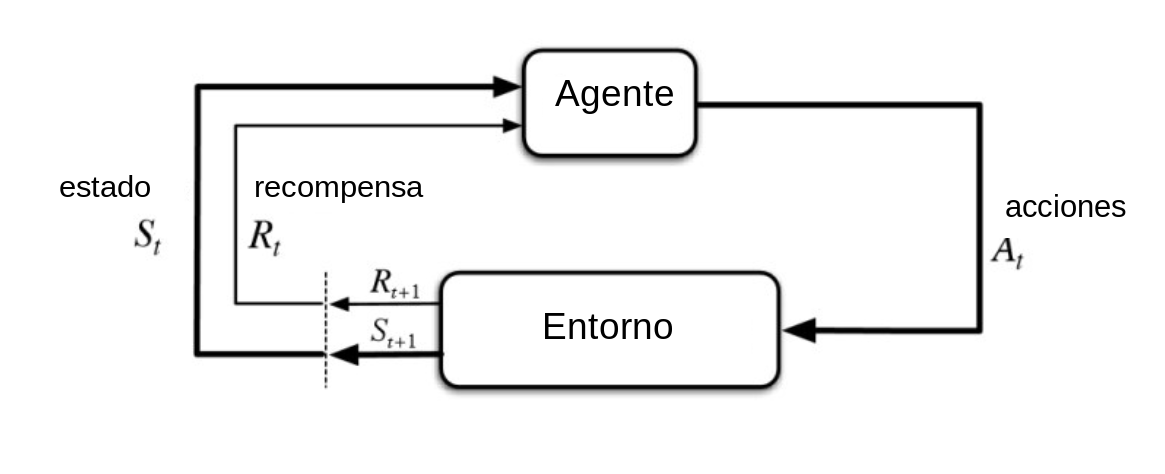
\includegraphics[width=0.75\textwidth]{img/refuerzo}
            \caption{Esquema de una tarea de aprendizaje por refuerzo. Fuente: \cite{bhatt_2018} }
            \label{fig:refuerzo}
        \end{figure}

        
    \subsection{Aprendizaje Profundo}
    Dentro del campo de la inteligencia artificial y el aprendizaje automático se han implementado diversos tipos 
    de algoritmos con éxito en los tipos de tareas de aprendizaje mencionados anteriormente. La base teórica y los detalles 
    de implementación de estos algoritmos son muy variados, sin embargo, las redes neuronales artificiales han experimentado 
    un incremento en el interés en la investigación y en las aplicaciones muy importante. Tal es el éxito de las mismas 
    que se ha creado un subcampo exclusivo llamado aprendizaje profundo o \textit{deep learning}. El aprendizaje profundo 
    es un campo de la inteligencia artificial que se encarga de estudiar exclusivamente a las redes neuronales artificiales, 
    sus componentes, arquitectura y aplicaciones. El impresionante rendimiento de estos algoritmos reside principalmente en el 
    concepto de la representación que generan a partir de los datos que se procesan. 

    El aprendizaje profundo resuelve el problema del aprendizaje de representaciones al introducir representaciones que se 
    expresan en términos de otras representaciones más simples. Además, permite a una computadora construir conceptos complejos 
    a partir de conceptos más simples. Un ejemplo de la generación de estos conceptos o representaciones se puede apreciar en la 
    Figura(\ref{fig:representacion}).
    
    
    \begin{figure}[!h] 
        \centering
        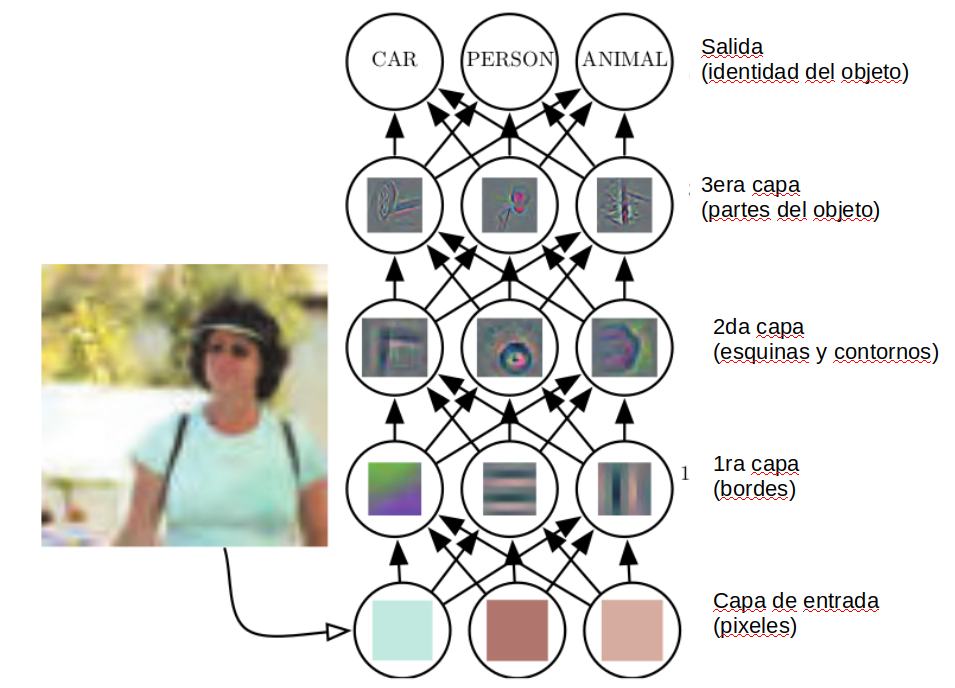
\includegraphics[width=0.75\textwidth]{img/representacion}
        \caption{Ilustración de un modelo de aprendizaje profundo. Las representaciones se generan en las capas ocultas y corresponden con características de distintos niveles de complejidad. Fuente: \cite{Goodfellow-et-al-2016} }
        \label{fig:representacion}
    \end{figure}

    A continuación, se procede a definir los conceptos más importantes de redes neuronales artificiales con los cuales se podrá 
    plantear la solución al problema de la conducción autónoma usando visión artificial.

        \subsubsection{Redes neuronales feedforward}
        Las redes neuronales feedforward o también llamadas perceptrón multicapa, son la base fundamental de los modelos 
        de aprendizaje profundo. El objetivo de una red neuronal feedforward es el de aproximar una función $f^\ast$. Por 
        ejemplo, para una tarea de clasificación, $y = f^\ast (\mathbf{x})$ mapea una entrada $\mathbf{x}$ a una categoría $y$.
        Una red neuronal feedforward define un mapeo $\mathbf{y} = f(\mathbf{x},\mathbf{W})$ y aprende el valor de los parámetros 
        $\mathbf{W}$ que resulten en la mejor aproximación\cite{Goodfellow-et-al-2016}.

        Este tipo de modelos son denominados feedforward debido a que la información fluye a por la función siendo evaluada 
        desde $\mathbf{x}$, a través de distintos cálculos intermedios definidos por $f$, hasta llegar a la salida $\mathbf{y}$.
        No existen conexiones de retroalimentación en las que la salidas del modelo se inyecten de nuevo a sí mismo. Las redes 
        neuronales que poseen este tipo de conexiones de retroalimentación son denominadas redes neuronales recurrentes.

        Para definir una red neuronal feedforward se puede comenzar definiendo un modelo basado en una combinación 
        lineal en conjunto con una función no lineal que toma la siguiente forma:

        \begin{equation}\label{eq:modelobase}
            y(\mathbf{x}, \textbf{W}) = f\left(\sum_{j=1}^M w_j  x_j\right)
        \end{equation}

        donde $f()$ es una función de activación no lineal. Esto lleva al modelo básico de una red neuronal que puede ser 
        descrita como una serie de transformaciones. Primero, se construyen $M$ combinaciones lineales de las variables 
        de entrada $x_1, \ldots , x_D$ donde $D$ es la dimensión del vector de entrada $\mathbf{x}$:
        
        \begin{equation}
            a_j = \sum_{i=1}^D w_{ji}^{(1)} x_i + w_{j0}^{(1)}
        \end{equation}

        donde $j = 1, \ldots , M$, y el superíndice $(1)$ indican que los correspondientes parámetros se encuentran en la 
        primera capa de la red. Los parámetros $w_{ji}^{(1)}$ se suelen conocer también con el nombre de \textit{pesos} y 
        los parámetros $ w_{j0}^{(1)}$ con el nombre de \textit{sesgos} o \textit{biases}. Las cantidades $a_j$ se conocen 
        como \textit{activaciones}, y cada una de ellas es luego transformada usando una función no lineal y derivable conocida 
        como la \textit{función de activación} $h()$ para luego obtener:

        \begin{equation}
            z_j = h(a_j)
        \end{equation}

        Estas cantidades corresponden con la salida de la capa y también se suelen referir por el nombre de  \textit{unidades ocultas}.
        Las funciones no lineales $h()$ pueden escogerse dependiendo a diversos criterios de rendimiento o de comportamiento. Siguiendo
        a la Ecuación(\ref{eq:modelobase}), las unidades ocultas se pueden volver a procesar con una combinación lineal y función 
        de activación en una segunda capa:

        \begin{equation}
            a_k = \sum_{j=1}^M w_{kj}^{(2)} z_j + w_{k0}^{(2)}
        \end{equation}

        donde $k = 1, \ldots, K$ y $K$ corresponden con el número de salidas de la segunda capa. Finalmente, si se considera a 
        esta capa como la capa de salida, podemos transformar las activaciones de la segunda capa con una función de activación. 
        Normalmente, para una tarea de regresión, la función de activación es una función identidad, es decir $y_k = a_k$. Para 
        una tarea de clasificación binaria, en cambio, la función de activación es una función sigmoide:

        \begin{equation}
            y_k = \sigma(a_k)
        \end{equation}

        donde
        
        \begin{equation}\label{eq:sigmoide}
            \sigma(a) = \frac{1}{1 + e^{-a}}    
        \end{equation}
        
        Finalmente, se pueden combinar las etapas en una función general de la red que, para una salida sigmoidal, toma la 
        siguiente forma:

        \begin{equation}\label{eq:reddoscapas}
            y_k(\mathbf{x}, \mathbf{W}) = \sigma \left( \sum_{j=1}^M w_{kj}^{(2)} h \left( \sum_{i=1}^D w_{ji}^{(1)} x_i + w_{j0}^{(1)} \right) + w_{k0}^{(2)} \right)
        \end{equation}

        De esta manera, se define una red neuronal de dos capas a partir de la combinación lineal de las entradas y las unidades 
        ocultas con los parámetros o pesos de la red transformados por funciones de activación no lineal. La arquitectura de la 
        red definida en la Ecuación(\ref{eq:reddoscapas}) se puede visualizar en la Figura(\ref{fig:reddoscapas}) donde se observa claramente las relaciones que se 
        han definido anteriormente en forma gráfica y la naturaleza del flujo en una sola dirección (feerforward) de los datos 
        desde la entrada hasta la salida. En este caso, la red neuronal analizada es una red neuronal con una capa oculta.

        \begin{figure}[!h] 
            \centering
            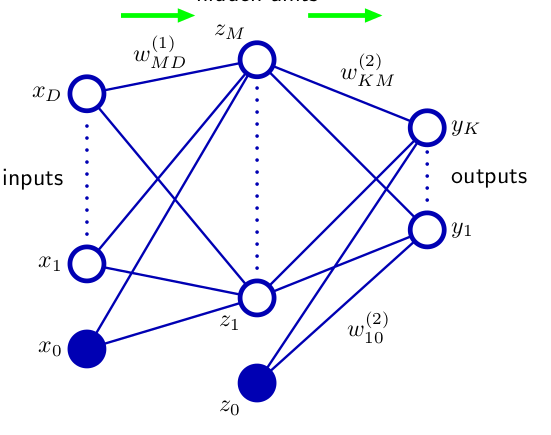
\includegraphics[width=0.75\textwidth]{img/reddoscapas}
            \caption{Diagrama de la red neuronal de dos capas correspondiente a la Ecuación(\ref{eq:reddoscapas}). Fuente: \cite{Bishop2006} }
            \label{fig:reddoscapas}
        \end{figure}
        
        \subsubsection{Funcion de costo}
        La función de costo es una función que permite definir el rendimiento de una red neuronal con respecto a las 
        predicciones esperadas a la salida. Un aspecto importante en el diseño de una red neuronal es la elección adecuada 
        de la función de costo. 

        La función de costo o función de error, se define de manera similar al caso del ajuste de curvas. Es decir, se desea 
        minimizar una suma de errores cuadráticos. Dado un conjunto de entrenamiento compuesto por un conjunto de vectores 
        de entrada $\{\mathbf{x}_n \}$, donde $n = 1, \ldots , N$, junto con un conjunto de vectores objetivo $\{\mathbf{t}_n \}$
        el objetivo es minimizar la función:

        \begin{equation}\label{eq:error}
            E(\mathbf{w}) = \frac{1}{2} \sum_{n=1}^N \{y(\mathbf{x}_n, \mathbf{w}) - t_n\}^2
        \end{equation}

        donde el valor de $\mathbf{w}$ que minimice la función de error $E(\mathbf{w})$ será considerado como el mejor conjunto 
        de parámetros sobre el cual el modelo puede generalizar.

        \subsubsection{Entrenamiento usando gradientes y retropropagación} \label{sec:gradientes}

        Una vez definidos con claridad los componentes básicos de una red neuronal feedforward y cómo es el proceso del flujo 
        de la información desde la entrada $\mathbf{x}$ hasta la salida $\mathbf{y}$, solamente queda especificar el procedimiento 
        necesario para ajustar los parámetros o pesos de la red $\mathbf{W}$. Para este cometido, el método más usado es el 
        de la retropropagación o \textit{backpropagation}, popularizado a partir del paper de Rumelhart \cite{rumelhart1986learning} 
        y ampliamente usado en la actualidad en la mayoría de las redes neuronales. La retropropagación tiene el objetivo de 
        encontrar los gradientes, en específico, se desea encontrar el gradiente de de la función de costo o error con respecto 
        a los parámetros $\nabla_{\mathbf{W}}E(\mathbf{W})$. Si se toma en cuenta que una red neuronal feedforward puede tener 
        varias capas ocultas, la gradiente de la función de costo está en función de los parámetros y funciones de activación 
        de cada capa, por tanto, se necesita usar la regla de la cadena para poder encontrar estos gradientes intermedios.

        Sea $y = g(x)$ y $z = f(g(x)) = f(y)$ dos funciones reales con argumento real, la regla de la cadena define lo siguiente:

        \begin{equation}
            \frac{dz}{dx} = \frac{dz}{dy} \frac{dy}{dx}
        \end{equation}

        Se puede generalizar la anterior expresión para casos fuera de una variable escalar donde $x \in \mathbb{R}^m$, 
        $y \in \mathbb{R}^n$, $g$ mapea de $\mathbb{R}^m$ a $\mathbb{R}^n$ y $f$ mapea de $\mathbb{R}^m$ a $\mathbb{R}$,
        si $\mathbf{y} = g(\mathbf{x})$ y $\mathbf{z} = g(\mathbf{y})$, entonces:

        \begin{equation}
            \frac{dz}{dx_i} =\sum_j \frac{dz}{dy_j} \frac{dy_j}{dx_i}
        \end{equation}

        en notación vectorial, sería equivalente a lo siguiente:

        \begin{equation}
            \nabla_{\mathbf{x}}z = \left( \frac{\partial \mathbf{y}}{\partial \mathbf{x}} \right)^T \nabla_{\mathbf{y}} z
        \end{equation}

        donde $\frac{\partial \mathbf{y}}{\partial \mathbf{x}}$ es el jacobiano $n \times m$ de $g$. Lo importante aqui 
        es recordar que en una función multivariable, el gradiente proporciona la dirección hacia donde la función crece 
        más rapidamente, esta intuición es fundamental para poder actualizar los pesos de la red en una etapa posterior.

        El concepto fundamental de la retropropagación es encontrar estos gradientes de manera secuencial, partiendo desde 
        la capa de salida hasta llegar a la capa de entrada. 

            \paragraph{Actualización de los parámetros de la red}
            La importancia de hallar los gradientes de la red con respecto a los pesos reside en que son justamente 
            los gradientes los que proporcionan la información de la evolución de los pesos con respecto de la función 
            de error y en qué dirección se encuentra el mínimo. En la Figura(\ref{fig:gradsup}) se puede ver cómo, para 
            una combinación arbitraria de pesos $\mathbf{w}_C$ el gradiente de la función de error $\nabla E$ indica 
            la direccion de máximo crecimiento de la superficie

            \begin{figure}[!h] 
                \centering
                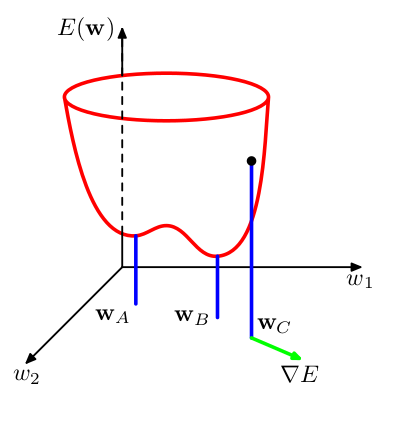
\includegraphics[width=0.55\textwidth]{img/gradsup}
                \caption{Visualización de la función de error $E(\mathbf{w})$ como una superficie. El punto $\mathbf{w}_A$ es un mínimo local y el punto $\mathbf{w}_B$ es el mínimo global. Fuente: \cite{Bishop2006} }
                \label{fig:gradsup}
            \end{figure}

            La actualización de los parámetros dados los gradientes de la red se puede realizar de distintas formas, pero una 
            de las más comunes es el algoritmo llamado \textit{Descenso de gradiente}, donde, de forma iterativa, se 
            va actualizando los pesos restando una medida del gradiente de la siguiente manera:

            Dicho de otro modo, en el descenso de gradiente, se avanza un pequeño paso en la dirección opuesta al gradiente 
            para avanzar hacia el mínimo:

            \begin{equation}
                \mathbf{w}^{(\tau + 1)} = \mathbf{w}^{(\tau)} - \alpha \nabla E(\mathbf{w}^{(\tau)})
            \end{equation}

            donde el parametro $\alpha > 0$ se conoce como la razón de aprendizaje o \textit{learning rate}. Después de 
            cada actualización, el gradiente es recalculado para poder encontrar los nuevos pesos y el proceso se repite 
            hasta encontrar el punto donde $\nabla E = 0$, lo que quiere decir que se ha llegado al mínimo. Usualmente, por 
            la naturaleza de la superficie de la función de error y diversos errores en el cálculo en una computadora, el número 
            de iteraciones se limita en base a cierto parámetro de rendimiento.

            Tradicionalmente, el algoritmo de descenso de gradiente se evalúa sobre todo el conjunto de datos de entrenamiento, 
            este tipo de descenso de gradiente es llamado \textit{batch gradient descent}, una \textit{pasada} por todo el conjunto 
            de entrenamiento se denomina usualmente una \textit{época}. La principal desventaja es que la 
            actualización de los pesos de la red neuronal solamente se actualiza una sola vez en cáda época; esto representa una 
            dificultad en tiempo de procesamiento y memoria cuando se procesan conjuntos de datos muy grandes. Se han desarrollado 
            versiones alternativas al \textit{batch gradient descent} que mejoran su desempeño y son más tratables con 
            conjuntos de datos muy grandes:

            \begin{itemize}
                \item \textbf{\textit{Stochastic Gradient Descent.}} Refiere a que la actualización de los pesos en cada muestra procesada, es decir, que los pesos se actualizan $n$ veces en una época.
                \item \textbf{\textit{Mini-batch Gradient Descent.}} Es una mezcla del descenso de gradiente tradicional y el descenso de gradiente estocástico, en este caso, las muestras se alimentan al algoritmo en \textit{mini-batches} o muestras de tamaño pequeño.
            \end{itemize}
        
            \paragraph{Adam}
            Adam, abreviación de \textit{Adaptive Moment Estimation}, es un algoritmo de optimización alternativo al descenso de 
            gradiente que utiliza promedios tanto de los gradientes como los momentos de segundo orden de los gradientes \cite{kingma2014adam}. Dados 
            los parámetros $\mathbf{w}^{(\tau)}$ y la función de error $E^{(\tau)}$, la actualización de parámetros de acuerdo 
            a Adam se da mediante las siguientes expresiones:

            \begin{align}
                m_w^{(\tau + 1)} &= \beta_1 m_w^{(\tau)} + (1 - \beta_1) \nabla_w E^{(\tau)} \nonumber \\
                v_w^{(\tau + 1)} &= \beta_2 m_w^{(\tau)} + (1 - \beta_2) (\nabla_w E^{(\tau)})^2 \nonumber \\
                \hat{m}_w &= \frac{m_w^{(\tau + 1)}}{1 - (\beta_1)^{(\tau + 1)} } \nonumber \\
                \hat{v}_w &= \frac{v_w^{(\tau + 1)}}{1 - (\beta_2)^{(\tau + 1)} } \nonumber \\
                w^{(\tau + 1)} &= w^{(\tau)} - \alpha \frac{\hat{m}_w}{\sqrt{\hat{v}_w} + \epsilon} \label{eq:adam}
            \end{align}

            Donde $m_w$ representa a los momentos de primer orden y $v_w$ representa a los momentos de segundo orden. Adam 
            tiene los siguientes hiperparámetros:

            \begin{itemize}
                \item $\alpha$ es la razón de aprendizaje, análogo al caso del descenso de gradiente tradicional.
                \item $\beta_1$ es la razón de decaimiento exponencial para el estimado de los momentos de primer orden.
                \item $\beta_2$ es la razón de decaimiento exponencial para el estimado de los momentos de segundo orden.
                \item $\epsilon$ es un escalar pequeño usado para prevenir una posible división entre cero.
            \end{itemize}

            La introducción de los estimados de los momentos de primer y segundo orden de los gradientes permiten que 
            se tome en cuenta el \textit{ímpetu} con el que los gradientes cambian en el proceso de entrenamiento lo cual 
            evita que pueda sobrepasar el mínimo y garantiza su convergencia a mayor velocidad que la de una actualización 
            con un descenso de gradiente tradicional.
            

        \subsubsection{Funciones de activación}
        Se ha estudiado con mucho detalle la naturaleza de la función de activación $f()$, introducida en la 
        Ecuación(\ref{eq:modelobase}), analizando fundamentalmente dos aspectos: su contribución a la generación 
        de representaciones internas en las capas ocultas de la red neuronal, así como también su comportamiento 
        de sus gradientes con relación a la etapa de aprendizaje, tal como se ha visto en la Sección(\ref{sec:gradientes}), 
        donde se ha establecido claramente que el papel de la función de activación y sus gradientes es fundamental para 
        el proceso de retropropagación y ajuste de los pesos de la red. Una guía con algunos criterios puede 
        encontrarse en \cite{mhaskar1994choose}, de donde se rescatan los siguientes aspectos a la hora de escoger una 
        función de activación:
        \begin{itemize}
            \item Que modele de forma no lineal la naturaleza de una representación interna fácil de interpretar.
            \item Que sea derivable en todo el rango de trabajo.
        \end{itemize}

        Tomando en cuenta lo anterior, se han generado diversas tendencias en la aplicación de funciones de activación y a 
        continuación se analizarán las más relevantes para este proyecto.
            \paragraph{Función sigmoide}\label{sec:sigmoide}
            Esta función ha sido introducida en la Ecuación(\ref{eq:sigmoide}) y representa, históricamente, la función 
            más utilizada en las primeras redes neuronales artificiales porque modela de manera aproximada, una respuesta 
            característica de las neuronas del cerebro \cite{narayan1997generalized}, pero sobre todo, porque posee las dos características mencionadas 
            anteriormente: naturaleza no lineal y diferenciable. Otra característica llamativa, es que se puede interpretar 
            a la salida como una función de probabilidad, pues sus valores van desde $0$ a $1$, como se puede apreciar 
            en la Figura(\ref{fig:sigmoide}). Usualmente se incluye un parámetro adicional para controlar el \textit{radio de activación}
            que hace que la función responda con más o menos sensibilidad a su entrada.

            \begin{figure}[!h] 
                \centering
                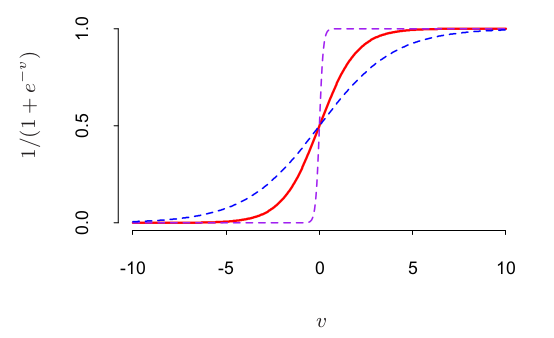
\includegraphics[width=0.75\textwidth]{img/sigmoide}
                \caption{Gráfico de la función sigmoide $\sigma(v) = 1 / (1 + e^{(-v)})$ (curva roja), y dos variaciones con un radio de activación de la forma $\sigma(sv)$ con valores $s=1/2$ (curva azul) y $s=10$ (curva púrpura) . Fuente: \cite{Goodfellow-et-al-2016} }
                \label{fig:sigmoide}
            \end{figure}
            
            Pese a las características anteriormente mencionadas, la función sigmoide tiene una gran desventaja: el llamado 
            \textit{desvanecimiendo de gradientes} \cite{hochreiter1998vanishing}. Este fenómeno ocurre cuando la activación 
            de una capa oculta tiene valores muy altos o muy negativos, se puede apreciar en la Figura(\ref{fig:sigmoide}), que 
            para estos valores, la derivada tiene un valor muy pequeño, aproximándose a cero mientras más grandes sean los valores.
            Este fenómeno ocasiona que, mientras se realiza la retropropagación de gradientes, dado que el gradiente tiene un valor 
            muy bajo, el ajuste en los pesos sea mínimo, deteniendo así el aprendizaje de la neurona en la que ocurre el fenómeno.

            Esta dificultad se presenta especialmente cuando la red neuronal se compone de varias capas ocultas y 
            ha motivado el desarrollo de nuevas funciones de activación que no presenten esta limitación y puedan 
            mantener valores de gradientes adecuados durante el entrenamiento.
            
            Cabe resaltar que, pese a las dificultades con la propagación de los gradientes de la función sigmoide, ésta se suele 
            utilizar bastante en la capa de salida, cuando se trata de clasificación binaria, ya que representa de manera adecuada
            la noción de probabilidad, lo cual es deseable en este tipo de modelos.

            \paragraph{Función tangente hiperbólica} \label{sec:tanh}
            La función tangente hiperbólica o $tanh()$ se define mediante la siguiente expresión:

            \begin{equation}\label{eq:tanh}
                tanh(x) = \frac{e^x - e^{-x}}{e^x + e^{-x}}
            \end{equation}

            Esta función también cumple con los requisitos de no linealidad y de ser derivable, pero en este caso, el rango de 
            salida de la función $tanh()$ es desde $-1$ a $1$. Considerando el concepto de función de probabilidad que ofrece 
            la salida de la función sigmoide, la función tangente hiperbólica introduce el concepto de aceptación o negación 
            de una premisa, donde una premisa aceptada se acerca a 1 y una premisa rechazada se acerca a -1, el valor de 0, 
            indica indecisión. La función $tanh()$ se ha usado junto a su par sigmoide ampliamente en los inicios de las redes 
            neuronales para las activaciones de las capas ocultas, pero, tal como se puede observar en la Figura(\ref{fig:tanh}), 
            presenta la misma desventaja del desvanecimiendo de gradientes, dado que para valores muy grandes, la derivada se 
            aproxima a cero.

            \begin{figure}[!h] 
                \centering
                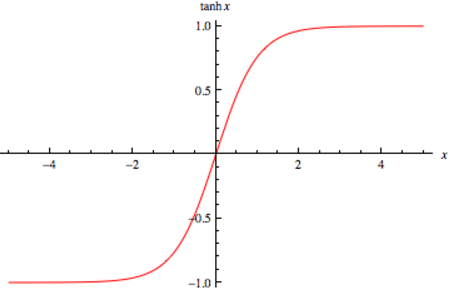
\includegraphics[width=0.75\textwidth]{img/tanh}
                \caption{Gráfico de la función tangente hiperbólica $tanh(x) = \frac{e^x - e^{-x}}{e^x + e^{-x}}$. Fuente: \cite{wang_2016} }
                \label{fig:tanh}
            \end{figure}

            En la actualidad, para implementaciones de redes neuronales profundas, el uso de las funciones sigmoide y tangente 
            hiperbólica en las capas ocultas está ampliamente desaconsejado por los problemas anteriormente planteados. En su 
            lugar se ha generado nuevos tipos de funciones de activación que presentan características bastante favorables 
            para el aprendizaje y ajuste de pesos basados en gradientes.

            \paragraph{Unidad Lineal Rectificada - ReLU}
            Introducida por primera vez en el año 2010 por Nair y Hinton, las Unidades Lineales Rectificadas o ReLU, se 
            propusieron para mejorar el rendimiento de un tipo especial de red neuronal: las máquinas restringidas de Boltzman 
            (RMB, por sus siglas en inglés) \cite{nair2010rectified}, pero pronto, ganarían gran popularidad también en las 
            redes neuronales feedforward y en redes neuronales convolucionales como se puede apreciar en \cite{krizhevsky2012imagenet}.
            
            La función ReLU se define de la siguiente manera:

            \begin{equation}\label{eq:relu}
                g(x) = max\{0,x\}
            \end{equation}

            Tal como se puede apreciar, la característica más importante de la función ReLU es su simplicidad pues es muy 
            similar a una función identidad, la diferencia es que ReLU toma el valor de cero para todos los valores de $x$ que 
            sean negativos. Esto resuelve el problema del desvanecimiendo de gradientes pues garantiza que el gradiente 
            tenga un valor razonable si la entrada está activa y además sea consistente.

            \begin{figure}[!h] 
                \centering
                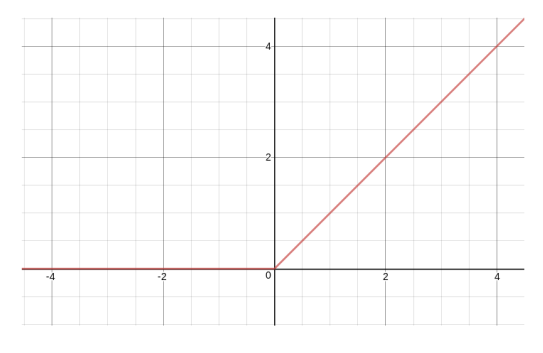
\includegraphics[width=0.75\textwidth]{img/relu}
                \caption{Gráfico de la ReLU. Fuente: \cite{wang_2016} }
                \label{fig:relu}
            \end{figure}

            Sin embargo, dado que la función ReLU tiene una gradiente nula para valores negativos es de vital importancia 
            que se garantice la existencia de gradientes positivos, aunque sea pequeños durante la inicialización y las capas 
            previas.

        \subsubsection{Diseño de Arquitectura e hiperparámetros de una red neuronal}
        Como se ha podido ver en las secciones anteriores, la característica más importante de una red neuronal es que es capaz
        de generar representaciones internas a partir de los datos y la retropropagación de los gradientes, lo que ha finalizado la era 
        de la ``ingeniería de características'' donde se necesitaba conocimiento experto para elegir las representaciones adecuadas y cómo calcularlas, sin embargo, esto 
        ha llevado a que el diseño de las redes se enfoque en otros aspectos como la arquitectura y otros parámetros externos 
        que definen el modelo de la red. Por arquitectura de la red, se entiende a la estructura general de la red neuronal, 
        el número de capas, el número de unidades o neuronas por cada capa y cómo las unidades y capas se conectan entre sí.

        La gran parte de las redes neuronales estan organizadas en grupos de unidades llamadas capas, asimismo, las capas se 
        ordenan de manera encadenada siendo cada capa una función de la capa que la precede, esto se ha establecido para una red de 
        dos capas en la Ecuación(\ref{eq:reddoscapas}) en su forma general, pero, se puede expresar el modelo de forma vectorial
        de la siguiente manera:

        \begin{align}
            \mathbf{h}^{(1)} &= g^{(1)} \left( \mathbf{W}^{(1)T}\mathbf{x} + \mathbf{b}^{(1)} \right) \\
            \mathbf{h}^{(2)} &= g^{(2)} \left( \mathbf{W}^{(2)T}\mathbf{h}^{(1)} + \mathbf{b}^{(2)} \right)
        \end{align}

        En términos de redesn neuronales, la cantidad de unidades en cada capa se denomina el ancho o \textit{width} 
        y la cantidad de capas se denomina profundidad o \textit{depth}.

            \paragraph{Hiperparámetros}
            Tanto la profundidad como el ancho de la red, son parámetros que se deben escoger en base a ciertos criterios, 
            éstos parámetros son externos a los parámetros o pesos $\mathbf{W}$ de la red neuronal, por lo que se demoninan
            hiperparámetros. Aparte del ancho y profundidad, en el diseño de una red neuronal se consideran las siguientes 
            variables:

            \begin{itemize}
                \item Razón de aprendizaje $\alpha$.
                \item Funciones de activación.
                \item Tamaño del \textit{mini-batch}.
                \item Número de épocas de entrenamiento.
                \item Algoritmo optimizador (Ejemplo: Descenso de gradiente).
                \item Función de costo.
            \end{itemize}

            Los hiperparámetros deberán ser escogidos de manera cuidadosa, pero debido a la gran complejidad y poca predictibilidad
            del comportamiento de una red neuronal profunda normalmente se eligen en conjunto con un proceso de prueba y error, 
            analizando las curvas de aprendizaje y rendimiento en conjuntos de datos de validación y prueba.

    \subsection{Redes Neuronales Convolucionales}
    Las redes neuronales convolucionales son un tipo especializado de red neuronal que 
    sirven para procesar datos de tipo "grilla" \cite{Goodfellow-et-al-2016}. Algunos ejemplos 
    de datos de tipo grilla que se pueden mencionar son los siguientes:
    \begin{itemize}
        \item \textbf{Series de tiempo.} Grilla de una dimensión tomados en intervalos regulares de tiempo.
        \item \textbf{Imágenes digitales.} Grilla de pixeles de dos o más dimensiones (Escala de grises, RGB).
    \end{itemize}

    Las también llamadas redes convolucionales, han demostrado un éxito impresionante en diversas 
    aplicaciones prácticas especialmente en el campo de la visión por computador y el procesamiento de texto y lenguaje natural. 
    El término ``red neuronal convolucional'' proviene del hecho de que en este tipo 
    de redes neuronales se utiliza una operación matemática llamada \textbf{convolución}, siendo la convolución 
    una operación lineal especializada para procesar datos de tipo grilla.

    En los párrafos posteriores, se procede a describir la operación de convolución en el contexto de 
    redes neuronales, pues, no siempre la definición de la misma corresponde con el concepto de convolución
    usado en distintos campos de la ciencia y la ingeniería.

        \subsection{Operación de convolución}
        En su forma más general, la convolución es una operación entre dos funciones reales y su definición se puede introducir
        usando el concepto de un promedio ponderado. Sea una función $x(t)$ dependiente del tiempo, 
        tanto $x$ como $t$ son números reales; en este caso, la función $x$ puede entenderse como una serie de medidas
        en un instante de tiempo $t$. Considérese una segunda función de ponderación $w(\tau)$ donde $\tau$ es la antiguedad 
        de una medida. Si se aplica la función de ponderación en cada instante de tiempo, se puede obtener una nueva función 
        definida por:
        \begin{equation}
            s(t) = \int x(\tau)w(t - \tau) d\tau
        \end{equation} 
        Esta operación es llamada la \textit{operación de convolución} y es denotada tradicionalmente con un asterisco:
        \begin{equation}
            s(t) = (x\ast w)(t)
        \end{equation}
        En el ejemplo de la ponderación, $w$ debe ser una función de densidad de probabilidad válida, o la salida no podrá
        ser considerada como un promedio ponderado. Además, $w$ también debe ser $0$ para cualquier $t<0$, esta última 
        característica se denomina comunmente como el principio de ``causalidad''. En general, la convolución está 
        definida para cualquier función en la cual la integral anteriormente declarada esté definida y puede ser 
        usada para otros propósitos aparte de promedios ponderados.

        Hablando en términos de una red neuronal convolucional, el primer argumento (en el ejemplo, la función $x$) 
        es comunmente referido como la \textbf{entrada}, y el segundo argumento ($w$, en el ejemplo) es referido 
        como el \textbf{kernel}. La salida, a su vez, es normalmente referida como el \textbf{mapa de características}.
        
        Por su parte, cuando se trata de señales digitales, como los datos en una computadora, el tiempo tiene una 
        naturaleza discreta, es decir, que los datos estarán disponibles en intervalos regulares de tiempo. En este 
        caso, el índice de tiempo $t$ puede tomar solamente valores enteros y, entonces, es válido asumir 
        que tanto $x$ como $w$ estan definidos solamente para valores enteros de $t$. De este modo, 
        se puede definir la convolución discreta:
        \begin{equation}
            s(t) = (x \ast w)(t) = \sum_{\tau=-\infty}^{\infty}x(\tau)w(t-\tau)
        \end{equation}

        En el contexto de las aplicaciones de aprendizaje automático o, más específicamente, aprendizaje profundo,
        la entrada es usualmente un arreglo multidimensional de datos, y el kernel es usualmente un arreglo 
        multidimensional de parámetros que se adaptan en el proceso de aprendizaje. 

        \subsubsection{Procesamiento de imágenes con redes neuronales convolucionales}
        La operación de convolución se usa frecuentemente sobre datos con más de una dimensión. Las imágenes digitales 
        son un perfecto ejemplo de un arreglo multidimensional de datos. Una imagen digital se representa mediante una
        matriz con filas y columnas, donde cada elemento se denomina pixel y contiene información acerca de la intensidad
        o luminancia, para una imagen en escala de grises o el nivel de color para distintos canales en una imagen a color.
        Si se toma el ejemplo de la imagen en escala de grises, se tiene una entrada o imagen bidimensional $I$ con un
        kernel bidimensional correspondiente $K$:

        \begin{equation} \label{eq:conv2d}
            S(i,j)=(I\ast K)(i,j) = \sum_{m} \sum_{n} I(m,n)K(i-m,j-n)
        \end{equation}

        Dado que la convolución es conmutativa, se puede reescribir la ecuación \ref{eq:conv2d} como:

        \begin{equation}
            S(i,j)=(K\ast I)(i,j) = \sum_{m} \sum_{n} I(i-m,j-n)K(m,n)
        \end{equation}

        Frecuentemente, la última fórmula es la más utilizada en librerías de aprendizaje profundo 
        por su sencillez en la implementación en un sistema computacional, esto, dado que existe menos 
        variación en el rango de valores válidos de $m$ y $n$. En la Figura(\ref{fig:convolucion}), se 
        puede apreciar una visualización de la operación de convolución aplicada a una imagen. 


        \begin{figure}[!h] 
            \centering
            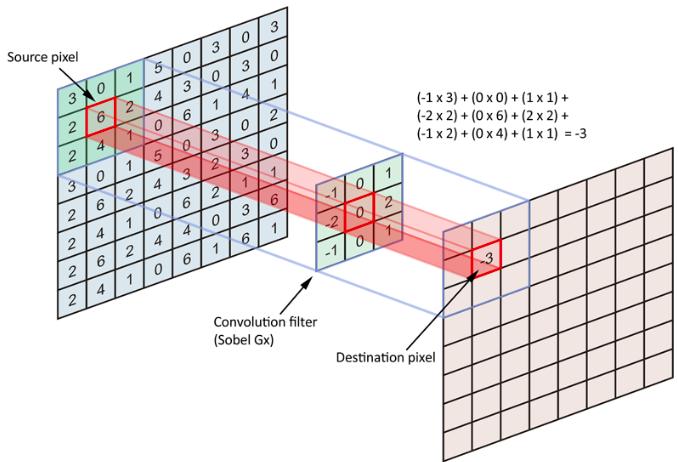
\includegraphics[width=0.75\textwidth]{img/convolucion}
            \caption{Visualización de la operación de convolución sobre una imagen digital. Fuente: \cite{cornelisse_2018} }
            \label{fig:convolucion}
        \end{figure}


        

        \subsubsection{Aprendizaje de representaciones internas}
        Una de las preguntas clave en la visión por computador es el cómo generar una buena y significativa
        representación interna de una imagen, dado que la mayor parte de la imagen corresponde con pixeles que no 
        aportan mucha información relevante a la tarea asignada. Por ejemplo, si se quisiera detectar 
        un rostro dentro de una imagen, normalmente se suele encontrar una representación que ayude a aislar solamente 
        las porciones de la imagen que pueden contener el rostro, tales como la búsqueda de contornos, bordes y 
        características típicas de un rostro. Antes de la aparición de las redes convolucionales, estas representaciones 
        se hallaban de manera manual y gracias al conocimiento de expertos en el área del procesamiento de imágenes. 
        La definición de características y mapas de características era comunmente conocida como la 
        \textit{ingeniería de características}, en la cual los expertos creaban descriptores para tareas específicas con 
        una gran inversión de tiempo en la sintonización fina de los mismos. 

        % TODO: poner el ejemplo de viola jones 

        En contraste con el anterior enfoque, las redes convolucionales generan sus propias representaciones internas
        de manera automática gracias al aprendizaje de los parámetros de cada uno de los kernels que componen las distintas 
        capas de la red neuronal. En principio, las redes convolucionales se inspiraron en el trabajo de Hubel y Wiesel 
        sobre la corteza visual primaria de un gato\cite{lecun2010convolutional}. En dicho trabajo, se logró identificar células simples que respondían
        de manera sobresaliente a distintas orientaciones con campos receptivos locales. Éstas células receptivas simples 
        se pueden corresponder con los kernels de convolución usados en las redes convolucionales por la sencillez y la 
        localidad de su campo de receptividad.

        Posteriormente, las redes convolucionales ganaron una gran popularidad debido a su rendimiento en tareas de 
        clasificación de imágenes y detección y reconocimiento de objetos en imágenes. El primer hito de su capacidad 
        para procesar imágenes de manera efectiva fue en concurso de clasificación de imágenes de ImageNet, donde 
        el equipo de Geoffrey Hinton logró sobrepasar el mejor resultado en precisión de clasificación por un gran márgen 
        usando una arquitectura de red convolucional \cite{krizhevsky2012imagenet}. En este trabajo, se pudo apreciar con 
        gran detalle las ventajas del enfoque del aprendizaje de representaciones internas en una red convolucional.

        \begin{figure}[!h] 
            \centering
            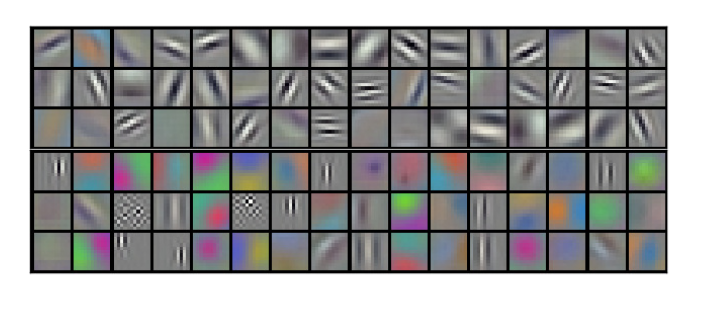
\includegraphics[width=0.75\textwidth]{img/fmap_imagenet}
            \caption{Kernels convolucionales de tamaño $11 \times 11 \times 3$ en la primera capa convolucional. Fuente: \cite{krizhevsky2012imagenet} }
            \label{fig:fmap_imagenet}
        \end{figure}
            
        Tal como se puede apreciar en la Figura(\ref{fig:fmap_imagenet}), en la primera capa convolucional, 
        los kernels de convolución corresponden con representaciones básicas en una imagen como la búsqueda de 
        bordes en distintas orientaciones, esto va acorde a lo establecido anteriormente en el modelo de 
        la corteza visual de un gato. Puede decirse entonces que las redes convolucionales emulan, en cierto modo, 
        al proceso biológico de visión en animales.

 
    \subsection{Sistemas de Aprendizaje Fin a Fin}
    Los sistemas de aprendizaje fin a fin refieren a sistemas complejos que se conciben, modelan y entrenan 
    como un conjunto para resolver cierto problema en vez de tratarse de forma separada por módulos. En términos
    de redes neuronales, los sistemas de aprendizaje fin a fin refieren a redes neuronales complejas, compuestas 
    por distintos componetes y tipos de unidades que usualmente tratan un problema de aprendizaje en su totalidad.
    
    En contraste con el desarrollo de los sistemas de aprendizaje tradicionales, tal como se pudo apreciar 
    en la Sección(\ref{sec:problema}) donde cada etapa del proceso debía ser cuidadosamente diseñada y evaluada por alguien 
    con la experiencia suficiente en el área, los sistemas fin a fin, dejan la responsabilidad de encontrar 
    las representaciones internas adecuadas al proceso de entrenamiento de la red neuronal en sí. Las representaciones
    adecuadas son generadas a partir del proceso de aprendizaje y ajuste de pesos en las distintas capas ocultas de la red 
    neuronal. Usualmente, las redes neuronales para aplicaciones de aprendizaje fin a fin se componen de varias etapas 
    de distinta naturaleza, de acuerdo al problema que se intenta resolver. 

    Los sistemas de aprendizaje fin a fin han demostrado ser una alternativa bastante llamativa debido a que presentan 
    las siguientes ventajas:

    \begin{itemize}
        \item \textbf{Diseño simplificado.} El diseño de un 
        sistema fin a fin es mucho menos demandante en cuestión de tiempo y conocimiento experto, la extracción de características
        no necesita ser una etapa elaborada por un experto pues se generará automáticamente.
        \item \textbf{Entrenamiento centralizado.} Dado que se trata de una sola red neuronal profunda que se incorporará en 
        el flujo de trabajo, el entrenamiento de la misma se realiza de forma única para todo el sistema.
        \item \textbf{Flexibilidad.} Debido a que el proceso de diseño solamente introduce criterios generales para la tarea 
        deseada, los sistemas fin a fin pueden ser fácilmente adaptados para realizar otras tareas en el futuro. Las iteraciones 
        en el diseño y entrenamiento no requieren de mucho tiempo ni esfuerzo. 
        \item \textbf{Modularidad.} La naturaleza de las representaciones internas generadas en las redes neuronales profundas 
        permite que las mismas se puedan reutilizar en otras tareas o arquitecturas.
    \end{itemize}

    Gracias a las ventajas anteriormente descritas, los avances en el desarrollo de sistemas 
    fin a fin han tenido particular éxito en las siguientes áreas:

    \begin{itemize}
        \item Reconocimiento de voz \cite{graves2014towards}.
        \item Control de brazos robóticos \cite{levine2016end}.
        \item Conduccion autónoma. \cite{bojarski2016end}.
    \end{itemize}

    En el presente proyecto, se utilizarán los conceptos de aprendizaje profundo, redes convolucionales y aprendizaje 
    fin a fin para diseñar un sistema de conducción autónoma.

\section{Robots móviles y locomoción con ruedas}
Un robot móvil es una máquina electromecánica con ciertos niveles de autonomía definida que son capaces de moverse 
y navegar por un entorno. Las ruedas aprovechan la fricción y el contacto con el suelo para hacer que el robot pueda moverse. 
Si se considera un vehículo ideal, donde las ruedas no se deslizan hacia los costados y mantienen contacto con el suelo en 
todo momento, para que exista un movimiento debe existir un punto alrededor del cual cada rueda sigue una trayectoria circular.
Este punto es conocido como el Centro Instantáneo de Rotación o Curvatura (ICC). En la práctica, el ICC se puede identificar de manera 
sencilla porque es el punto que yace en una linea coincidente con el eje de rotación de cada rueda. El ICC define la curvatura 
de la trayectoria que sigue el robot en cada momento. En la Figura(\ref{fig:icc}), se puede apreciar una configuración compatible 
con el movimiento sin deslizamiento de las ruedas y una configuración incompatible.

\begin{figure}[!h] 
    \centering
    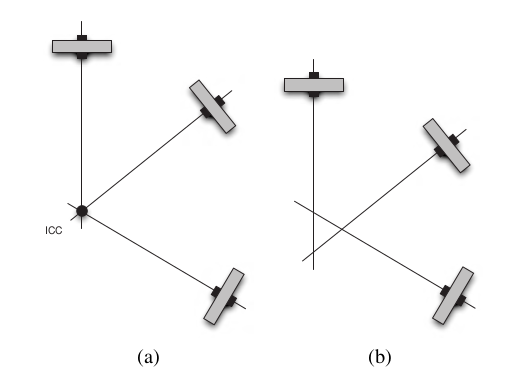
\includegraphics[width=0.75\textwidth]{img/icc}
    \caption{Centro instantáneo de curvatura o ICC. (a) Arreglo compatible con el movimiento, (b) arreglo incompatible con el movimiento. Fuente: \cite{krizhevsky2012imagenet} }
    \label{fig:icc}
\end{figure}


La existencia del ICC es una condición necesaria pero no suficiente para el movimiento de un robot con ruedas, también las 
velocidades de cada rueda deben ser consistentes con la rotación rígida del vehículo en su conjunto. Un robot localizado en 
un plano tiene tres grados de libertad: una posición $(x,y)$ y una orientación $\theta$. Este conjunto de parámetros $(x,y,\theta)$ 
es comúnmente denominado la pose del robot en el plano.

Los robots móviles usualmente no poseen un control absoluto sobre los tres parámetros de su pose y deben realizar diversas 
maniobras para poder alcanzar una pose en particular. Estas restricciones en el control de su movimiento se conocen como 
restricciones no holonómicas. 

    \subsection{Modelo de locomoción de Ackerman}
    Es el tipo de locomoción encontrada en la mayoría de los automóviles domésticos. En este modelo, las ruedas frontales estan 
    direccionadas y pueden rotar distintos ángulos de tal manera que sus ejes de rotación se intersectan en el ICC. La rueda 
    direccionada interna debe rotar un ángulo un poco mayor que la externa para que la condición se cumpla Figura(\ref{fig:ackerman}).


    \begin{figure}[!h] 
        \centering
        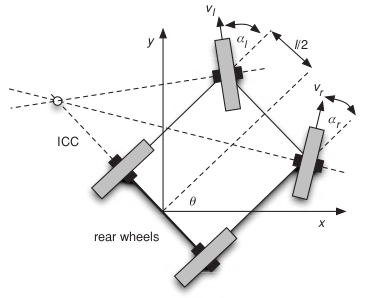
\includegraphics[width=0.75\textwidth]{img/ackerman}
        \caption{Modelo cinemático de Ackerman. Fuente: \cite{GregoryMcGillUniversity2010} }
        \label{fig:ackerman}
    \end{figure}

    La locomoción de Ackerman es la preferida en vehículos de gran tamaño, los cuales están diseñados para operar en carreteras
    existentes y soportar una carga considerable. Normalmente, el tamaño del vehículo permite incorporar una gran cantidad 
    de sensores y sistemas de control. 
        \subsubsection{Cinemática directa}
        El vehículo rota alrededor de un punto que yace en la linea que pasa por el eje trasero una distancia $R$ del centro 
        del vehículo donde

        \begin{equation*}
            R - l/2 = d \tan{(\pi / 2 - \alpha_l)}
        \end{equation*}

        Para que las ruedas puedan rodar la segunda rueda de dirección debe ser rotada un ángulo $\alpha_r$, donde 

        \begin{equation*}
            R + l/2 = d \tan{(\pi / 2 - \alpha_r)}
        \end{equation*}

        En general, las cuatro ruedas viajan por el suelo a velocidades diferentes y al especificar la velocudad de una sola rueda
        se puede obtener las velocidades de las restantes. El modelo de locomoción de Ackerman es muy sofisticado y ha sido 
        estudiado ampliamente. Para los objetivos del presente proyecto, se puede simplificar el modelo sin perder ninguna 
        propiedad importante.

    \subsection{Modelo de la bicicleta o triciclo} \label{sec:triciclo}
    Los modelos de la bicicleta y el triciclo tienen modelos cinemáticos muy similares. Un triciclo típico tiene tres ruedas: 
    dos ruedas de tracción traseras y una rueda de dirección delantera. El movimiento del robot es controlado por la dirección 
    $\alpha$ y la velocidad $v$.
    \begin{figure}[!h] 
        \centering
        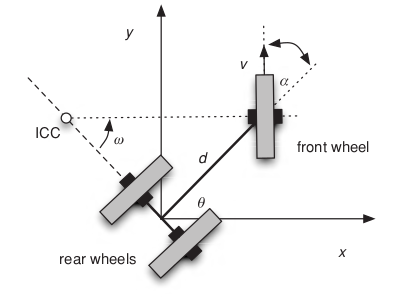
\includegraphics[width=0.75\textwidth]{img/triciclo}
        \caption{Modelo cinemático del triciclo. Fuente: \cite{GregoryMcGillUniversity2010} }
        \label{fig:triciclo}
    \end{figure}    

        \subsubsection{Cinemática directa}
        Si la rueda de dirección se orienta en un ángulo $\alpha$ de la dirección hacia adelante, el triciclo rotará con una 
        velocidad angular $\omega$ con respecto al punto que yace a una distancia $R$ de la línea perpendicular que pasa 
        por el eje trasero donde $R$ y $\omega$ están dados por las siguientes expresiones:

        \begin{align}
            R       &= d \tan(\frac{\pi}{2} - \alpha) \\
            \omega  &= \sqrt{\frac{v}{d^2 + R^2}}
        \end{align}

        donde $d$ es la distancia desde la rueda frontal al eje trasero, como se observa en la Figura(\ref{fig:triciclo}).

    
    En el presente proyecto, se considerará el uso del modelo del triciclo definido en la Sección(\ref{sec:triciclo}) 
    por razones de simplicidad.


\chapter{Marco Práctico} \label{ch:m_practico}
\section{Arquitectura del sistema}
    \subsection{}
        \subsubsection{}
\section{Subsistema de Adquisición de Datos y Entrenamiento}
    \subsection{Descripción general del subsistema}
    \subsection{Módulo de adquisición de datos y operación manual}
    \subsection{Módulo de aumentación de datos y almacenamiento}
    \subsection{Módulo de Entrenamiento}
\section{Subsistema de Control y actuación}
    \subsection{Descripción general del subsistema}
    \subsection{Características del prototipo físico}
    \subsection{Módulo de potencia y sensado de tiempo real}
    \subsection{Módulo de la computadora de abordo}
    \subsection{Interfaces de comunicación}
    
\section{Subsistema de Inferencia y control autónomo}

% \chapter{Análisis y discusión de resultados}
\label{ch:resultados}
\section{Proceso de entrenamiento}\label{sec:analisistrain}
El primer paso para poder verificar la validez del sistema de predicción con la red neuronal es el análisis 
de las curvas de entrenamiento. Se puede extraer información valiosa acerca del rendimiento observando 
la naturaleza de dichas curvas. Se ha trabajado con el conjunto de datos explorado en la Sección(\ref{sec:dataset}) 
que cuenta con un total de 26356 muestras entre datos reales y datos aumentados. Se procede a explorar la naturaleza 
de las curvas de entrenamiento.
    
    \subsection{Análisis de las curvas de entrenamiento}

    Las curvas de entrenamiento representan una herramienta bastante valiosa a la hora de evaluar el proceso de entrenamiento 
    de un algoritmo de aprendizaje. A través de las mismas se puede extraer información sobre la convergencia del entrenamiento, 
    la evolución del mismo y también, gracias al proceso de validación cruzada, se puede analizar la presencia de sobreentrenamiento 
    en el sistema.

        \subsubsection{Error de entrenamiento}

        En la Figura(\ref{fig:trainloss}) se puede observar la evolución del error de entrenamiento para ambas arquitecturas implementadas. 
        %% foto de ejemplo
        \begin{figure}[!ht] 
            \centering
            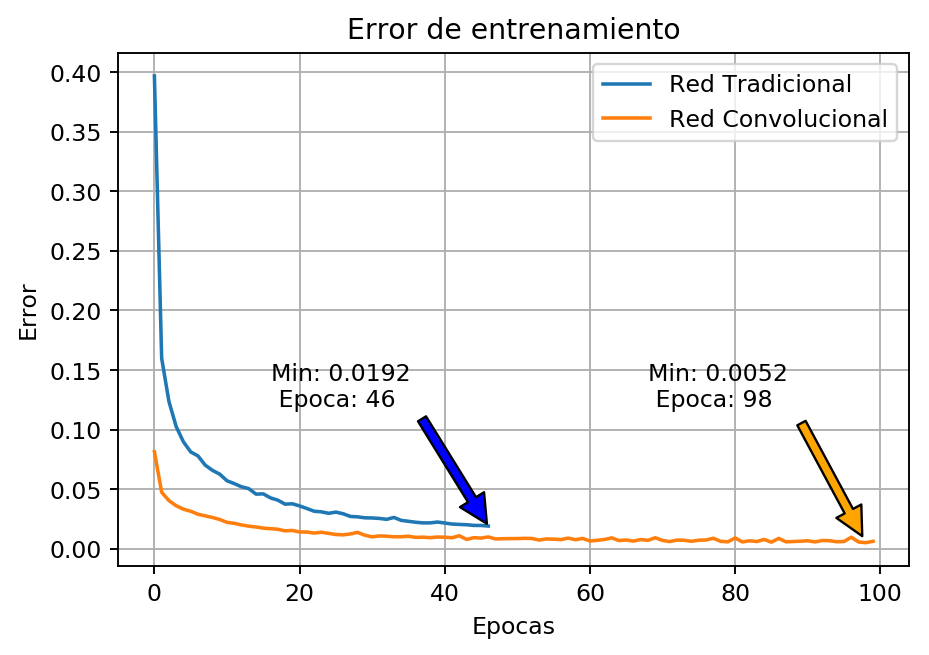
\includegraphics[width=0.75\textwidth]{img/trainloss}
            \caption[Error de entrenamiento]{Error de entrenamiento. Fuente: Elaboración propia. }
            \label{fig:trainloss}
        \end{figure}

        Observando las curvas de error de entrenamiento se pueden realizar las siguientes observaciones con respecto a la red neuronal convolucional:

        \begin{itemize}
            \item \textbf{El error de entrenamiento inicial es menor:} Esto indica que la capacidad de ajuste de parámetros 
            es más eficaz en la red neuronal pues en la primera época es capaz de obtener un error de entrenamiento 7 veces 
            menor. A esta propiedad se le llama eficacia a nivel de muestras.
            \item \textbf{El error mínimo es menor:} Esto indica que la red convolucional se aproxima mejor al conjunto de 
            entrenamiento debido a las representaciones generadas por las capas convolucionales internas. En el caso de la red 
            tradicional, se puede observar que el mínimo se mantiene en un valor casi cuatro veces mayor que en la red convolucional. 
            Esto ocurre por la limitada capacidad de generar representaciones internas de imágenes de una red con capas densamente conectadas pues 
            en las primeras capas se trabaja a nivel de pixeles mientras que en una capa convolucional se procesan mapas de características.
            \item \textbf{Convergencia más rápida:} La convergencia hacia el valor mínimo comienza a notarse alrededor de la época número 20, 
            en contraste con la red tradicional que comienza a converger a partir de la época 35. La convergencia está directamente 
            relacionada con el tiempo de entrenamiento requerido por cada arquitectura.
        \end{itemize}

        Considerando los aspectos anteriormente mencionados, se puede observar claramente que el rendimiento en el conjunto 
        de entrenamiento de la red convolucional es superior al de la red tradicional.

        \subsubsection{Error de validación}
        Los resultados obtenidos en el análisis del error de entrenamiento no son suficientes para determinar si la red neuronal 
        convolucional tiene un mejor rendimiento general que la red tradicional. Para poder obtener un mejor panorama, se puede 
        usar el error de validación, que básicamente corresponde con el cálculo del error de predicción de la red en cada época 
        contra un conjunto de datos nunca antes visto, llamado el conjunto de validación. El error de validación brinda información 
        acerca de la capacidad de generalización de la red. En la Figura(\ref{fig:valloss}), se puede observar la evolución del error de 
        validación para ambas arquitecturas.

        \begin{figure}[!ht] 
            \centering
            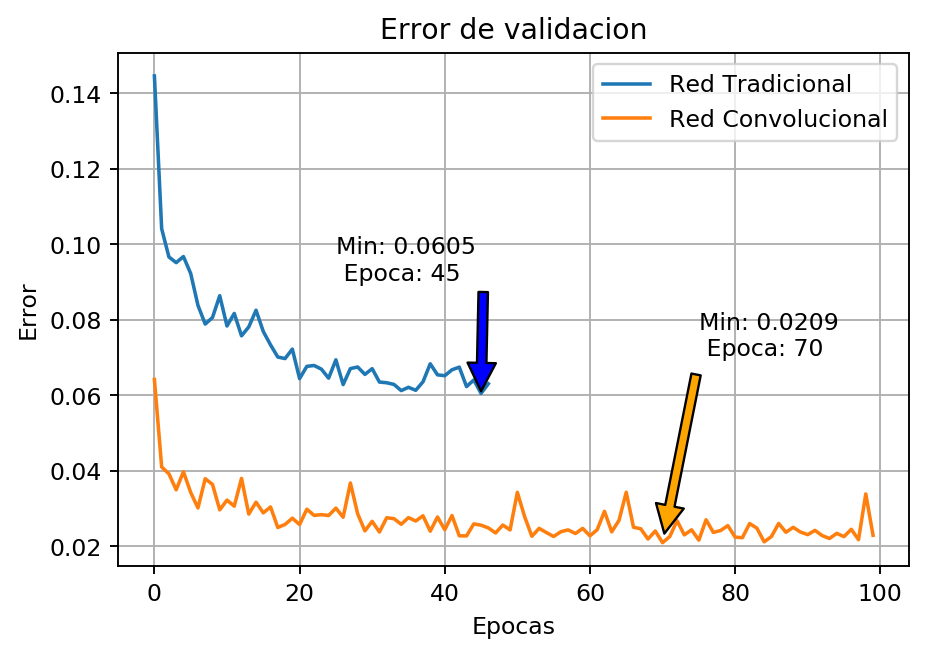
\includegraphics[width=0.75\textwidth]{img/valloss}
            \caption[Error de validación]{Error de validación. Fuente: Elaboración propia. }
            \label{fig:valloss}
        \end{figure}
        
        De manera similar al análisis de las curvas del error de entrenamiento se puede realizar algunas observaciones concernientes
        a las curvas del error de validación:

        \begin{itemize}
            \item \textbf{El error de inicial es menor:} Es un indicativo que la capacidad de generalización de la red convolucional 
            es mucho mayor desde la primera época. Es decir, que con solamente una pasada por el conjunto de entrenamiento, tiene una 
            capacidad mayor de realizar predicciones cercanas a la realidad en casos nunca antes vistos, como son las muestras del
            conjunto de validación.
            \item \textbf{El error mínimo es menor:} En este caso, el error de validación mínimo indica que la capacidad de generalización 
            de la red convolucional es mayor al de la red tradicional. Si el error de la red convolucional fuera mayor, esto podría indicar 
            sobreentrenamiento de la red. En este caso, se puede observar que se llega al mínimo alrededor de la época número 70.
            \item \textbf{Convergencia:} La convergencia del error de validación indica que ambas redes neuronales no están siendo 
            sobreentrenadas, sin embargo, los valores del error son menores para la red convolucional mostrando que su rendimiento 
            y capacidad de generalización son mayores al de una red tradicional.
        \end{itemize}
    
    \subsection{Puntajes y errores en el conjunto de prueba}\label{sec:scores}
    Más allá del análisis de las curvas de entrenamiento, se puede evaluar al modelo entrenado en base a sus puntajes o 
    \textit{scores} definidos para este tipo de tarea. En el presente proyecto, se evaluó a los modelos en base a 
    los puntajes definidos en la Tabla(\ref{tbl:metrics}).


    % Please add the following required packages to your document preamble:
    % \usepackage{booktabs}
    % \usepackage{graphicx}
    \begin{table}[!h]
        \centering
        \resizebox{0.65\textwidth}{!}{%
        \begin{tabular}{@{}|c|c|c|@{}}
        \toprule
        \textbf{Métrica} & \textbf{Nombre} & \textbf{Definición} \\ \midrule
        MSE & Error Cuadrático Medio & Ecuación(\ref{eq:mse}) \\ \midrule
        MAE & Error Absoluto Medio & Ecuación(\ref{eq:mae}) \\ \midrule
        $R^2$ & Coeficiente de Determinación & Ecuación(\ref{eq:r2}) \\ \bottomrule
        \end{tabular}%
        }
        \caption{Métricas para la evaluación del modelo}
        \label{tbl:metrics}
    \end{table}

    Los resultados de la evaluación del modelo sobre el conjunto de prueba se pueden observar en la Tabla(\ref{tbl:testscores}) donde se 
    nota claramente la superioridad en todas las métricas de la red neuronal convolucional. 

    % Please add the following required packages to your document preamble:
    % \usepackage{booktabs}
    % \usepackage{graphicx}
    \begin{table}[!h]
        \centering
        \resizebox{0.45\textwidth}{!}{%
        \begin{tabular}{@{}|c|c|c|c|@{}}
        \toprule
        \textbf{Modelo} & \textbf{MSE} & \textbf{MAE} & $\mathbf{R^2}$ \\ \midrule
        Tradicional & 0.0254 & 0.0976 & 0.9278 \\ \midrule
        Convolucional & 0.0160 & 0.0872 & 0.9484 \\ \bottomrule
        \end{tabular}%
        }
        \caption{Evaluación de puntajes sobre el conjunto de prueba}
        \label{tbl:testscores}
    \end{table}

    Se puede observar en detalle algunas predicciones en la Tabla(\ref{tbl:predsample}), de la cual se debe rescatar principalmente el signo 
    de la predicción que indica la dirección de viraje correcta.

    % Please add the following required packages to your document preamble:
    % \usepackage{booktabs}
    % \usepackage{graphicx}
    \begin{table}[]
        \centering
        \resizebox{0.55\textwidth}{!}{%
        \begin{tabular}{@{}|c|c|c|c|@{}}
        \toprule
        \textbf{Valor real} & \textbf{Predicción} & \textbf{Diferencia} & \textbf{\begin{tabular}[c]{@{}c@{}}Predicción de\\ signo correcta\end{tabular}} \\ \midrule
        -0.297 & -0.243 & 0.054 & \checkmark \\ \midrule
        1.0 & 0.921 & 0.079 & \checkmark \\ \midrule
        0.149 & 0.22 & 0.07 & \checkmark \\ \midrule
        -1. & -0.968 & 0.032 & \checkmark \\ \midrule
        -0. & 0.069 & 0.069 & $\times$ \\ \bottomrule
        \end{tabular}%
        }
        \caption{Muestra de predicciones de la red convolucional}
        \label{tbl:predsample}
    \end{table}

    Nótese que la única predicción errónea en dirección de la muestra tiene que ver con un valor nulo, sin embargo, el error 
    de la predicción es muy similar a las otras muestras.
\section{Pruebas}\label{sec:analisistest}

Pese a que se ha validado la efectividad de la red neurona convolucional analizando el error en los conjuntos de entrenamiento, 
validación y prueba, es necesario realizar un análisis cualitativo de los resultados en base a pruebas de campo del modelo.
Se procede a analizar el rendimiento y generación de representaciones internas de la red neuronal convolucional dadas 
nuevas muestras que ingresan al modelo. Se presta especial atención al signo de la predicción.

    \subsection{Análisis del rendimiento en pruebas de campo}
    Dada la naturaleza de la tarea, es importante analizar de manera detallada las predicciones que está arrojando la red 
    neuronal para casos nuevos. Se ha grabado una nueva sesión de muestras para evaluar el rendimiento del sistema. Los 
    resultados de esta evaluación se pueden observar en la Figura(\ref{fig:testimg}).

    \begin{figure}[!h] 
        \centering
        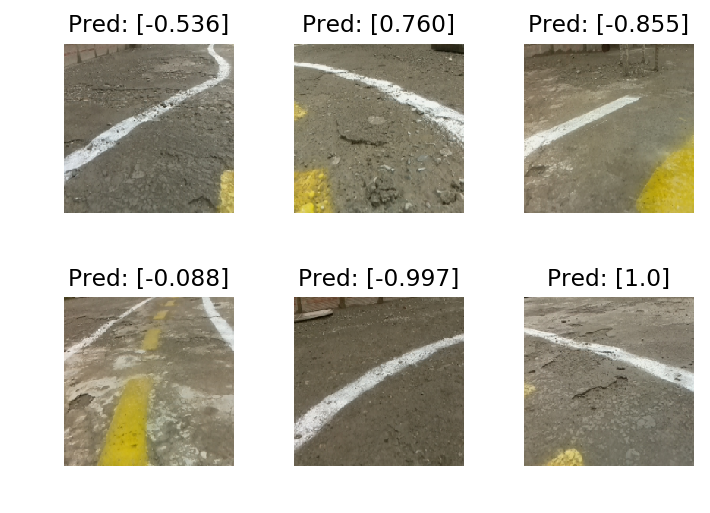
\includegraphics[width=0.75\textwidth]{img/testimg}
        \caption[Ejemplos de predicción de la red convolucional]{Ejemplos de predicción de la red convolucional. Fuente: Elaboración propia. }
        \label{fig:testimg}
    \end{figure}

    De la anterior figura, es importante tomar en cuenta que el signo de la predicción indica la dirección en la que se debe 
    mover el vehículo dada la imagen de la carretera. El signo correcto de la predicción es fundamental para el funcionamiento 
    adecuado del sistema. Una predición con signo errado puede llevar a la inestabilidad del sistema. 

    También se puede notar que la predicción es correcta pese a que no se puedan observar ambas líneas delimitadoras del carril 
    e incluso, en casos en los que la línea no cruza completamente la imagen.

    \subsection{Análisis de representaciones internas}\label{sec:representaciones}

    Ya se ha discutido la importancia de las capas convolucionales para la generación automática de representaciones internas 
    de los datos de entrada. En la Figura(\ref{fig:filtros1}) se puede visualizar los filtros de la primera capa convolucional.
    
    \begin{figure}[!h] 
        \centering
        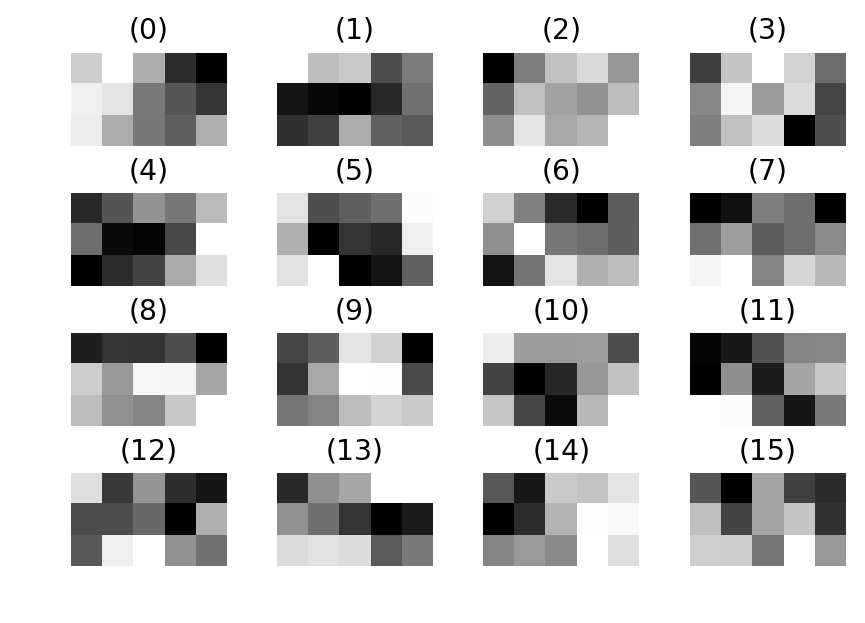
\includegraphics[width=0.65\textwidth]{img/filtros1}
        \caption[Filtros de la primera capa convolucional]{Filtros de la primera capa convolucional. Fuente: Elaboración propia. }
        \label{fig:filtros1}
    \end{figure}

    Es interesante analizar la naturaleza de los filtros generados en el proceso de aprendizaje. Por ejemplo, en el filtro 
    (\ref{fig:filtros1},0), se puede apreciar claramente que el filtro está dando importancia a bordes con una inclinación 
    hacia la derecha, de manera similar, el filtro (\ref{fig:filtros1},5) detecta bordes inclinados hacia la izquierda.

    
    \begin{figure}[!h] 
        \centering
        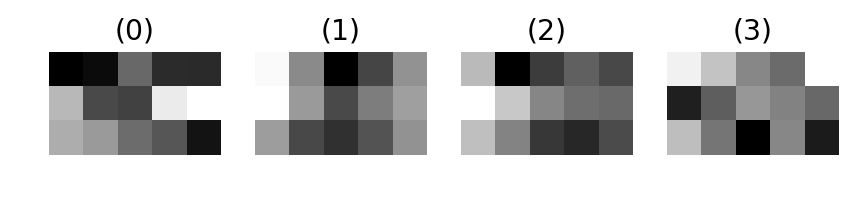
\includegraphics[width=0.65\textwidth]{img/filtros7}
        \caption[Filtros de la penúltima capa convolucional]{Filtros de la penúltima capa convolucional. Fuente: Elaboración propia. }
        \label{fig:filtros7}
    \end{figure}

    En el caso de los filtros de las capas superiores, se puede observar que las representaciones son mucho más abstractas. Por 
    ejemplo, en el filtro (\ref{fig:filtros7},0) se da importancia a activaciones que aparezcan a la derecna, en el 
    (\ref{fig:filtros7},2) a la izquierda y en el (\ref{fig:filtros7},4) a activaciones que aparecen a ambos lados, cuando 
    el vehículo está centrado en la carretera.

    Lo más importante en este análisis es resaltar el hecho de que la red neuronal ha generado estos filtros exclusivamente 
    mediante el proceso de aprendizaje basado en retropropagación de manera automática. En ningún momento en la etapa de diseño, 
    se ha incorporado algún criterio indicando que las líneas de la carretera tendrían bordes inclinados a la izquierda o derecha 
    o aparecerían a los costados de la imagen. Esto demuestra la impresionante capacidad de las redes neuronales convolucionales 
    para analizar imágenes de manera natural.

    Posteriormente, se puede analizar las activaciones que generan en las capas convolucionales algunas imágenes obtenidas 
    en la etapa de pruebas del prototipo. Se analizarán tres casos en los que la red establezca predicciones de 
    viraje a la izquierda, a la derecha y al centro.

        \subsubsection{Giro a la izquierda}
        En la Figura(\ref{fig:predizq}) se puede observar el paso de una imagen en la que el vehículo tiene que virar hacia la izquierda por 
        las capas convolucionales de la red neuronal. 

        \begin{figure}[!h] 
            \centering
            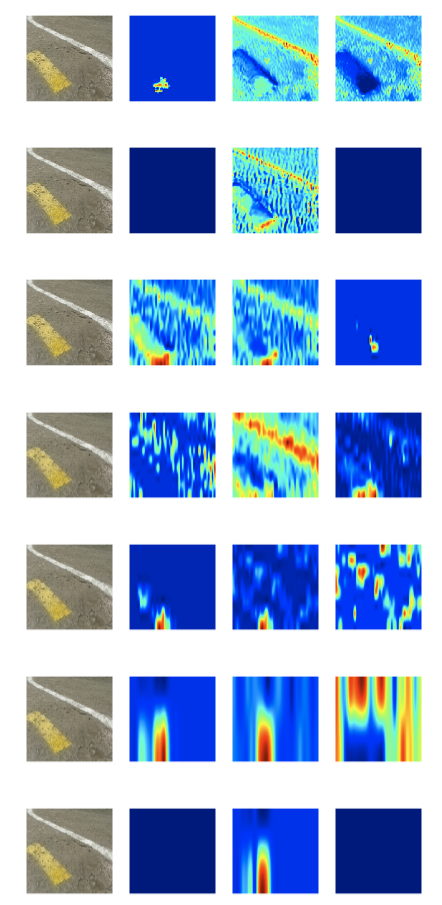
\includegraphics[width=0.60\textwidth]{img/predizq}
            \caption[Activaciones para una imagen con giro a la izquierda]{Activaciones para una imagen con giro a la izquierda, el valor de 
            la predicción es 1. Fuente: Elaboración propia. }
            \label{fig:predizq}
        \end{figure}

        Los mapas de características generados para esta imagen denotan activaciones con valor alto en las regiones donde estan 
        presentes las líneas de la carretera. A medida que se avanza en las capas convolucionales, se puede observar un máximo 
        en el lado izquierdo de la imagen. Este máximo corresponde con el valor de la predicción que se puede interpretar como un comando 
        de viraje máximo a la izquierda.
        

        \subsubsection{Giro a la derecha}
        En la Figura(\ref{fig:predder}) se puede observar el paso de una imagen en la que el vehículo tiene que virar hacia la derecha por 
        las capas convolucionales de la red neuronal. 

        \begin{figure}[!h] 
            \centering
            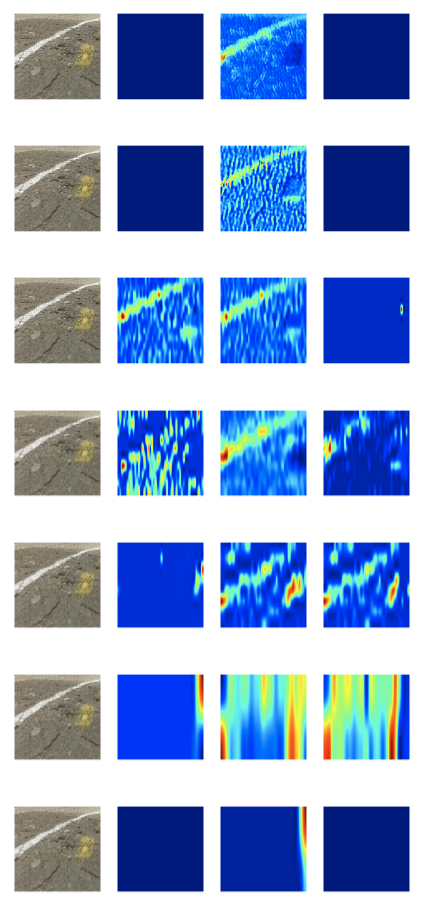
\includegraphics[width=0.60\textwidth]{img/predder}
            \caption[Activaciones para una imagen con giro a la derecha]{Activaciones para una imagen con giro a la derecha, el valor de 
            la predicción es -0.84. Fuente: Elaboración propia. }
            \label{fig:predder}
        \end{figure}

        Los mapas de características generados para esta imagen denotan activaciones con valor alto en las regiones donde estan 
        presentes las líneas de la carretera. A medida que se avanza en las capas convolucionales, se puede observar un máximo 
        en el lado derecho de la imagen. Este máximo corresponde con el valor de la predicción que se puede interpretar como un comando 
        de viraje a la derecha.


        \subsubsection{Conducir hacia adelante}
        En el caso en el que el vehículo se encuentre centrado, el comando de control debe aproximarse a cero, pues este 
        valor representa que se tiene que mantener la dirección actual. En la Figura(\ref{fig:predade}) se observa cómo el máximo se encuentra 
        cerca al centro de la imagen, lo que significa que el vehículo debe mantener su dirección. 


        \begin{figure}[!h] 
            \centering
            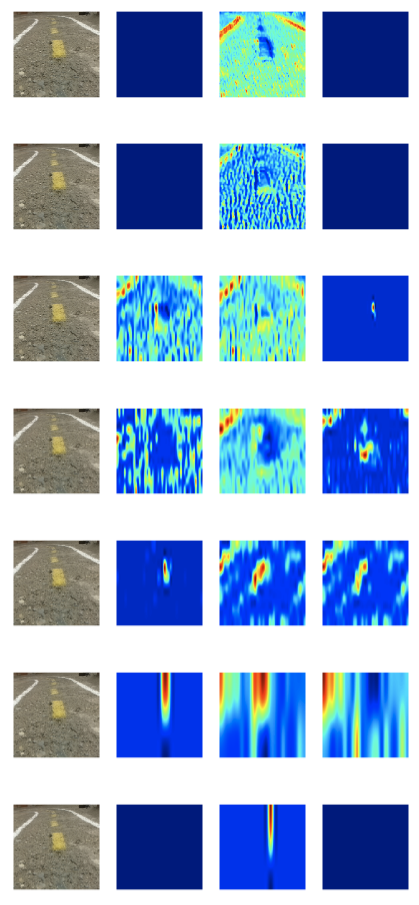
\includegraphics[width=0.60\textwidth]{img/predade}
            \caption[Activaciones para una imagen con dirección hacia adelante]{Activaciones para una imagen con dirección hacia adelante, el valor de 
            la predicción es -0.1. Fuente: Elaboración propia. }
            \label{fig:predade}
        \end{figure}

        De esta manera se ha podido observar la naturaleza del procesamiento que es capaz de hacer una red neuronal convolucional 
        y la forma en la que las representaciones internas que se generan en el aprendizaje son válidas para la 
        tarea de regresión.



% \chapter{Conclusiones y recomendaciones}
\label{ch:conclusiones}
\section{Conclusiones}
\section{Recomendaciones}

% \appendix
\chapter{Código Fuente}\label{aped.A}
Aún faltan cosas por decir.


% \lhead[\thepage]{REFERENCIAS}
\rhead[REFERENCIAS]{\thepage}

\cleardoublepage
\addcontentsline{toc}{chapter}{Bibliografía}
\bibliographystyle{IEEEtran}
\bibliography{referencias}
\cleardoublepage
% \chapter{Bibliografía}
\addcontentsline{toc}{chapter}{Bibliografía}
\bibliographystyle{IEEEtran}
\bibliography{referencias}


\end{document}
